\documentclass[12pt,a4paper]{article}

% ==================== FONT / ENCODING ====================
\usepackage[utf8]{inputenc}
\usepackage[T5]{fontenc}
\usepackage{mathptmx}

% ==================== TOÁN HỌC ====================
\usepackage{amsmath,amssymb,amsfonts,yhmath}
\numberwithin{figure}{subsection}
\numberwithin{table}{subsection}

% ==================== LAYOUT ====================
\usepackage[top=2cm, bottom=2cm, left=3cm, right=2cm]{geometry}
\usepackage{setspace}
\onehalfspacing

\usepackage{indentfirst}
\setlength{\parindent}{1.1cm}

% ==================== DANH SÁCH / BẢNG / HÌNH ====================
\usepackage{enumitem}
\usepackage[table]{xcolor}
\usepackage{booktabs}
\usepackage{array}
\usepackage{graphicx}
\usepackage{float}

% ==================== TIKZ ====================
\usepackage{tikz}
\usetikzlibrary{
    calc,
    arrows.meta,
    shadows,
    decorations.pathreplacing
}

% ==================== MÀU SẮC ====================
\definecolor{uehred}{RGB}{210, 50, 40}
\definecolor{uehteal}{HTML}{2D5D66}
\definecolor{uehorange}{HTML}{D96B42}
\definecolor{uehblue}{HTML}{1A408B}
\definecolor{vscodebg}{HTML}{1E1E1E}
\definecolor{vscodegreen}{HTML}{6A9955}
\definecolor{vscodetext}{HTML}{D4D4D4}
\definecolor{LightGray}{gray}{0.9}


\definecolor{genBlue}{RGB}{230, 240, 255}
\definecolor{genGreen}{RGB}{230, 255, 230}
\definecolor{genOrange}{RGB}{255, 240, 230}
\definecolor{lineBlue}{RGB}{60, 120, 200}
\definecolor{lineGreen}{RGB}{60, 160, 80}
\definecolor{lineOrange}{RGB}{210, 120, 50}

% ==================== TITLE / SECTION ====================
\usepackage{titlesec}
\titleformat{\section}{\Large\bfseries}{\thesection}{1em}{}
\titleformat{\subsection}{\large\bfseries}{\thesubsection}{1em}{}

% ==================== CÁC GÓI KHÁC CỦA FILE GỐC ====================
\usepackage{fontawesome5}
\IfFileExists{ex_test.sty}{\usepackage[solcolor]{ex_test}}{}
\usepackage{anyfontsize}
\usepackage{longtable}
\usepackage{makecell}
\usepackage{pdflscape}
\usepackage{hyperref}

\hypersetup{unicode, hidelinks, hypertexnames=false}
\graphicspath{{resources/}}

% ==================== MINTED: CODE PYTHON TỰ XUỐNG DÒNG ====================

\usepackage{minted}
\setminted{
    frame=lines,
    framesep=1mm,
    baselinestretch=1.0,
    bgcolor=lightgray!12,
    fontsize=\scriptsize,
    linenos,
    numbersep=6pt,
    breaklines=true,
    breakanywhere=true,
    autogobble=true
}

\renewcommand{\theFancyVerbLine}{
    \textcolor{gray!60!white}{\scriptsize\arabic{FancyVerbLine}}
}

% ==================== ALGORITHM: DÙNG BẢN BREAKABLE ====================
% Không dùng \begin{algorithm}[H] cho thuật toán dài nữa,
% vì algorithm là float và dễ bị nhảy nguyên khối sang trang sau.
\usepackage{algpseudocode}
\usepackage{caption}
\usepackage[most]{tcolorbox}
\tcbuselibrary{breakable}
\usepackage{tabularx}      % Bắt buộc cho môi trường tabularx và cột X


% ==================== LIÊN KẾT MÃ NGUỒN / DANH MỤC THUẬT TOÁN ====================
% Các đoạn mã nguồn hiện được hiển thị trực tiếp trong nội dung chính; macro cũ được giữ để tương thích nếu cần.
\newcommand{\sourcecodebox}[2]{%
\begin{center}
\begin{tcolorbox}[
    enhanced,
    breakable,
    colback=uehblue!3,
    colframe=uehblue!65!black,
    boxrule=0.6pt,
    arc=2mm,
    left=2mm,
    right=2mm,
    top=1.5mm,
    bottom=1.5mm,
    title={\faCode\ Mã nguồn minh họa},
    fonttitle=\bfseries
]
#1
\par\medskip
\centering
\hyperref[#2]{%
\tikz[baseline=(btn.base)]\node[fill=uehblue, rounded corners=3pt, inner xsep=8pt, inner ysep=4pt] (btn) {\textcolor{white}{\bfseries Nhấn vào đây để xem mã nguồn}};%
}
\end{tcolorbox}
\end{center}
}

\newcounter{breakablealgocounter}

\newenvironment{breakablealgorithm}[1]
{
    \refstepcounter{breakablealgocounter}
    \addcontentsline{loa}{appendixentry}{\protect\numberline{Thuật toán \thebreakablealgocounter}#1}
    \begin{tcolorbox}[
        breakable,
        enhanced,
        colback=white,
        colframe=black!55,
        sharp corners,
        boxrule=0.5pt,
        left=2mm,
        right=2mm,
        top=1mm,
        bottom=1mm,
        title={Thuật toán \thebreakablealgocounter. #1},
        fonttitle=\bfseries
    ]
}
{
    \end{tcolorbox}
}

% ==================== VIỆT HÓA ====================
\renewcommand{\contentsname}{Mục lục}
\renewcommand{\figurename}{Hình}
\renewcommand{\tablename}{Bảng}
\renewcommand{\refname}{Tài liệu tham khảo}
\renewcommand{\listfigurename}{Danh mục hình ảnh}
\renewcommand{\listtablename}{Danh mục bảng biểu}

% ==================== CUSTOM TOÁN HỌC ====================
\renewcommand{\ge}{\geqslant}
\renewcommand{\geq}{\geqslant}
\renewcommand{\le}{\leqslant}
\renewcommand{\leq}{\leqslant}

\newcommand{\tron}[1]{\left( #1 \right)}
\newcommand{\vuong}[1]{\left[ #1 \right]}
\newcommand{\nhon}[1]{\left\{ #1 \right\}}
\newcommand{\sieuto}[1]{\Big( #1 \Big)}


% Chèn hình an toàn: nếu thiếu file ảnh/PDF, LaTeX vẫn biên dịch và hiện khung thông báo.
\newcommand{\safeincludegraphics}[2][]{%
    \IfFileExists{#2}{\includegraphics[#1]{#2}}{%
        \fbox{\parbox{0.72\textwidth}{\centering \textit{Thiếu tệp hình:} \texttt{\detokenize{#2}}}}%
    }%
}


% Tiêu đề phụ lục kèm mô tả ngắn.
\newcommand{\appendixnote}[1]{\par\smallskip\noindent\textit{#1}\par\medskip}

% ==================== DANH MỤC PHỤ LỤC TỰ ĐỘNG ====================
% In trực tiếp danh sách hình, bảng, thuật toán và mã nguồn ở cuối báo cáo
% theo dạng mục lục có dấu chấm dẫn, số trang và hyperlink.
\makeatletter
\newcommand{\printappendixfigures}{\@starttoc{lof}}
\newcommand{\printappendixtables}{\@starttoc{lot}}
\newcommand{\printappendixalgorithms}{\@starttoc{loa}}

% Dòng tự động cho danh mục hình, bảng, thuật toán và mã nguồn.
% Danh mục hình/bảng vẫn lấy dữ liệu tự động từ \caption, nhưng hiển thị thêm tiền tố Hình/Bảng.
\renewcommand*{\l@figure}[2]{\@dottedtocline{1}{0em}{6.2em}{\figurename~#1}{#2}}
\renewcommand*{\l@table}[2]{\@dottedtocline{1}{0em}{6.2em}{\tablename~#1}{#2}}
\newcommand*{\l@appendixentry}{\@dottedtocline{1}{0em}{7.2em}}
\makeatother

% Môi trường mã nguồn minh họa trực tiếp trong nội dung chính.
% Theo yêu cầu trình bày: không dùng hộp tiêu đề, chỉ dùng minted dạng frame=lines
% với số dòng bên trái để mã nguồn gọn và giống phong cách tài liệu kỹ thuật.
\newcounter{codecounter}
\newenvironment{codeblock}[2]{%
    \refstepcounter{codecounter}%
    \phantomsection%
    \label{#1}%
    \par\smallskip
}{%
    \par\smallskip
}




\begin{document}
\pagenumbering{gobble}

% ==================== TRANG BÌA ====================
\begin{titlepage}

\begin{tikzpicture}[remember picture, overlay]
    \node[inner sep=0pt] at (current page.center) {
        \safeincludegraphics[width=1.1\paperwidth, height=1\paperheight]{resources/khung_pdf.pdf}
    };
\end{tikzpicture}

\centering
\vspace*{0.2cm}

{\small BỘ GIÁO DỤC VÀ ĐÀO TẠO} \\[0.2cm]
{\bfseries \large ĐẠI HỌC KINH TẾ TP HỒ CHÍ MINH (UEH)} \\[0.2cm]
{\bfseries \small TRƯỜNG CÔNG NGHỆ VÀ THIẾT KẾ} \\
\vspace{1cm} 

\safeincludegraphics[width=5cm]{resources/Logo_UEH_xanh.png} \\
\vspace{1cm} 

{\bfseries \Large ĐỒ ÁN MÔN HỌC} \\[0.5cm]
{\bfseries \large ĐỀ TÀI} \\[0.5cm]
\textcolor{uehred}{\bfseries \Large GIẢI BÀI TOÁN TỐI ƯU MẠNG/LUỒNG GIAO} \\[0.3cm]
\textcolor{uehred}{\bfseries \Large THÔNG DỰA TRÊN GIẢI THUẬT DI TRUYỀN} \\
\vspace{0.8cm}

\begin{flushleft}
\hspace{3.5cm} \textbf{Học Phần:} Trí Tuệ Nhân Tạo \\[0.2cm]
\hspace{3.5cm} \textbf{Danh Sách Nhóm}: \\[0.5cm]
\hspace{4.5cm} 1 \hspace{0.5cm} NGUYỄN HOÀNG ANH \\[0.2cm]
\hspace{4.5cm} 2 \hspace{0.5cm} LỮ VÕ HOÀNG PHÚC \\[0.2cm]
\hspace{4.5cm} 3 \hspace{0.5cm} NGUYỄN ĐỨC TRÍ \\[0.2cm]
\hspace{4.5cm} 4 \hspace{0.5cm} MINH THƯ \\
\end{flushleft}
\vspace{0.5cm} 

\begin{flushleft}
\hspace{3.5cm} \textbf{Chuyên Ngành:} KHOA HỌC DỮ LIỆU - \textcolor{uehred}{KỸ THUẬT} \\[0.1cm]
\hspace{3.5cm} \textcolor{uehred}{PHẦN MỀM} \\[0.2cm]
\hspace{3.5cm} \textbf{Khóa:} \textcolor{uehred}{K50} \\[0.8cm]
\hspace{3.5cm} \textbf{Giảng Viên:} Đặng Ngọc Hoàng Thành
\end{flushleft}

\vfill

{\bfseries \small Tp. Hồ Chí Minh, Ngày xx tháng 12 năm 2025}

\end{titlepage}

% ==================== TRANG MỤC LỤC ====================
\newpage
\tableofcontents
\thispagestyle{empty} 

% ==================== DANH MỤC THUẬT NGỮ VÀ KÝ HIỆU ====================
% ==================== TÓM TẮT VÀ LỜI CẢM ƠN ====================
\newpage
\thispagestyle{empty}

\section*{TÓM TẮT}
\phantomsection
\addcontentsline{toc}{section}{TÓM TẮT}

Đề tài nghiên cứu bài toán lập lộ trình phương tiện (Vehicle Routing Problem -- VRP) và ứng dụng Giải thuật Di truyền để tìm lời giải gần tối ưu trong thời gian chấp nhận được. Hệ thống xây dựng mô hình biểu diễn nhiễm sắc thể dựa trên chuỗi hoán vị khách hàng và các điểm phân cắt tuyến, kết hợp ma trận chi phí, hàm fitness, các toán tử chọn lọc, lai ghép, đột biến và cơ chế xử lý ràng buộc bằng hàm phạt. Ngoài mô hình VRP cơ bản, đồ án mở rộng sang CVRP và VRPTW nhằm phản ánh các ràng buộc thực tế về tải trọng và thời gian phục vụ. Kết quả thực nghiệm cho thấy mô hình có khả năng cải thiện lời giải qua nhiều thế hệ, trực quan hóa được quá trình hội tụ và hỗ trợ phân tích chất lượng tuyến đường thông qua giao diện người dùng.

\noindent\textbf{Từ khóa:} Vehicle Routing Problem, Genetic Algorithm, CVRP, VRPTW, optimization, logistics.

\vspace{1.2cm}

\section*{LỜI CẢM ƠN}
\phantomsection
\addcontentsline{toc}{section}{LỜI CẢM ƠN}

Nhóm chúng em xin gửi lời cảm ơn chân thành đến thầy Đặng Ngọc Hoàng Thành, giảng viên học phần Trí Tuệ Nhân Tạo, đã hướng dẫn và tạo điều kiện để nhóm thực hiện đồ án này. Trong quá trình nghiên cứu và xây dựng hệ thống, nhóm đã có cơ hội củng cố kiến thức về các bài toán tối ưu tổ hợp, Giải thuật Di truyền, mô hình hóa ràng buộc và trực quan hóa kết quả thuật toán.

Chúng em cũng xin cảm ơn Trường Công nghệ và Thiết kế -- Đại học Kinh tế TP. Hồ Chí Minh (UEH) đã cung cấp môi trường học tập và định hướng thực hành, giúp nhóm có điều kiện vận dụng kiến thức lý thuyết vào một bài toán có tính ứng dụng thực tế trong lĩnh vực logistics và tối ưu vận tải.

Do giới hạn về thời gian, kinh nghiệm nghiên cứu và phạm vi triển khai, đồ án khó tránh khỏi những thiếu sót nhất định. Nhóm chúng em rất mong nhận được những góp ý từ thầy để tiếp tục hoàn thiện mô hình, cải thiện chất lượng thực nghiệm và mở rộng hệ thống trong các hướng nghiên cứu tiếp theo.

\begin{flushright}
\textit{Nhóm thực hiện}
\end{flushright}
\newpage
\thispagestyle{empty}
\section*{DANH MỤC THUẬT NGỮ VÀ KÝ HIỆU}
\phantomsection
\addcontentsline{toc}{section}{DANH MỤC THUẬT NGỮ VÀ KÝ HIỆU TOÁN HỌC}

Phần này tóm tắt các thuật ngữ chuyên ngành và ký hiệu toán học được sử dụng trong Chương 1--7. Mục này chỉ đóng vai trò tra cứu nhanh trước khi đi vào nội dung chính, vì vậy không đưa vào mục lục chính của báo cáo.

\subsection*{Thuật ngữ chuyên ngành}
\renewcommand{\arraystretch}{1.22}
\begin{longtable}{|p{3.2cm}|p{10.8cm}|}
\hline
\textbf{Thuật ngữ} & \textbf{Diễn giải ngắn gọn} \\
\hline
\endfirsthead
\hline
\textbf{Thuật ngữ} & \textbf{Diễn giải ngắn gọn} \\
\hline
\endhead
VRP & \textit{Vehicle Routing Problem}: bài toán lập lộ trình cho đội xe nhằm phục vụ tập khách hàng với tổng chi phí thấp. \\
\hline
CVRP & \textit{Capacitated VRP}: biến thể VRP có ràng buộc tải trọng tối đa trên mỗi xe. \\
\hline
VRPTW & \textit{VRP with Time Windows}: biến thể VRP có ràng buộc cửa sổ thời gian phục vụ tại từng khách hàng. \\
\hline
MDVRP & \textit{Multi-Depot VRP}: biến thể VRP xét nhiều kho trung tâm hoặc nhiều điểm xuất phát. \\
\hline
GA & \textit{Genetic Algorithm}: giải thuật meta-heuristic mô phỏng quá trình tiến hóa tự nhiên thông qua chọn lọc, lai ghép và đột biến. \\
\hline
Chromosome & Cá thể/nhiễm sắc thể biểu diễn một lời giải ứng viên trong GA; trong đồ án gồm \texttt{genes} và \texttt{breaks}. \\
\hline
Genes & Chuỗi hoán vị các khách hàng, biểu diễn thứ tự ghé thăm trong không gian định tuyến. \\
\hline
Breaks & Các điểm phân cắt dùng để chia chuỗi \texttt{genes} thành nhiều tuyến tương ứng với nhiều xe. \\
\hline
Depot & Kho trung tâm hoặc điểm xuất phát/kết thúc của phương tiện. \\
\hline
Fitness & Giá trị độ thích nghi của cá thể. Với bài toán cực tiểu chi phí, fitness thường được ánh xạ nghịch đảo từ tổng chi phí. \\
\hline
Penalty & Chi phí phạt được cộng vào hàm mục tiêu khi lời giải vi phạm ràng buộc tải trọng hoặc thời gian. \\
\hline
Elitism & Cơ chế bảo tồn một số cá thể tốt nhất sang thế hệ kế tiếp để tránh làm mất nghiệm tốt. \\
\hline
Early Stopping & Cơ chế dừng sớm khi lời giải tốt nhất không còn cải thiện đáng kể sau một số thế hệ liên tiếp. \\
\hline
Stagnation & Hiện tượng thuật toán không cải thiện nghiệm tốt nhất trong một khoảng thời gian dài. \\
\hline
Heuristic & Quy tắc tìm kiếm kinh nghiệm, ưu tiên tạo lời giải tốt trong thời gian ngắn thay vì bảo đảm tối ưu tuyệt đối. \\
\hline
Meta-heuristic & Khung tìm kiếm cấp cao điều phối nhiều thao tác heuristic, ví dụ GA, Tabu Search, Simulated Annealing. \\
\hline
\end{longtable}

\subsection*{Ký hiệu toán học}
\renewcommand{\arraystretch}{1.22}
\begin{longtable}{|p{3.2cm}|p{10.8cm}|}
\hline
\textbf{Ký hiệu} & \textbf{Ý nghĩa} \\
\hline
\endfirsthead
\hline
\textbf{Ký hiệu} & \textbf{Ý nghĩa} \\
\hline
\endhead
$V$ & Tập tất cả các đỉnh trong mạng lưới, gồm depot và khách hàng. \\
\hline
$V_c$ & Tập khách hàng cần được phục vụ. \\
\hline
$D$ & Tập depot/kho trung tâm. \\
\hline
$n = |V_c|$ & Số lượng khách hàng trong bài toán. \\
\hline
$k$ & Số lượng phương tiện hoặc số tuyến tối đa. \\
\hline
$Q$ & Tải trọng tối đa của mỗi xe trong mô hình CVRP. \\
\hline
$q_i$ & Nhu cầu hàng hóa của khách hàng $i$. \\
\hline
$C_{ij}$ & Chi phí hoặc khoảng cách di chuyển từ điểm $i$ đến điểm $j$. \\
\hline
$C \in \mathbb{R}^{N \times N}$ & Ma trận chi phí giữa các điểm trong mạng lưới. \\
\hline
$B$ & Mảng các điểm phân cắt trong chromosome. \\
\hline
$\pi$ & Hoán vị các khách hàng trong chuỗi \texttt{genes}. \\
\hline
$[e_i,l_i]$ & Cửa sổ thời gian phục vụ của khách hàng $i$, gồm thời điểm sớm nhất và muộn nhất. \\
\hline
$t_i$ & Thời điểm xe đến hoặc bắt đầu phục vụ khách hàng $i$. \\
\hline
$s_i$ & Thời gian phục vụ tại khách hàng $i$ nếu mô hình có xét thời gian phục vụ. \\
\hline
$\mathcal{F}(x)$ & Hàm mục tiêu mở rộng của cá thể $x$, gồm chi phí gốc và chi phí phạt. \\
\hline
$f_{\text{cost}}(x)$ & Thành phần chi phí vận hành gốc của lời giải $x$. \\
\hline
$P(x)$ & Tổng chi phí phạt do vi phạm ràng buộc. \\
\hline
$\text{Fitness}(x)$ & Độ thích nghi của lời giải $x$; trong đồ án thường lấy dạng $1/\mathcal{F}(x)$. \\
\hline
$\sum$ & Ký hiệu tổng. Ví dụ $\sum_{i \in r} q_i$ là tổng nhu cầu của các khách hàng thuộc tuyến $r$. \\
\hline
$\forall$ & Ký hiệu ``với mọi''. Ví dụ $\forall k \in K$ nghĩa là với mọi xe thuộc tập xe $K$. \\
\hline
$\in$ & Ký hiệu thuộc tập. Ví dụ $i \in V_c$ nghĩa là khách hàng $i$ thuộc tập khách hàng. \\
\hline
$\cup$ & Phép hợp tập hợp; dùng khi ghép thêm tuyến hoặc phần tử vào một tập. \\
\hline
$\emptyset$ & Tập rỗng, thường dùng khi khởi tạo tập tuyến hoặc quần thể chưa có phần tử. \\
\hline
$|A|$ & Số phần tử của tập hoặc mảng $A$. \\
\hline
$\arg\min$ & Toán tử trả về đối tượng làm cho biểu thức đạt giá trị nhỏ nhất. Ví dụ $\arg\min_{d \in D}(C_{d,f}+C_{l,d})$ chọn depot có chi phí khứ hồi nhỏ nhất. \\
\hline
$\arg\max$ & Toán tử trả về đối tượng làm cho biểu thức đạt giá trị lớn nhất, thường dùng khi chọn cá thể có fitness cao nhất. \\
\hline
$\min,\max$ & Giá trị nhỏ nhất/lớn nhất của một biểu thức hoặc một tập giá trị. \\
\hline
$\mathcal{O}(\cdot)$ & Ký hiệu độ phức tạp tiệm cận, mô tả tốc độ tăng chi phí tính toán khi kích thước đầu vào tăng. \\
\hline
$\varepsilon$ & Hằng số dương rất nhỏ, thường dùng để tránh phép chia cho 0. \\
\hline
$\Delta$ & Độ thay đổi của một đại lượng, ví dụ dịch chuyển điểm phân cắt sang trái/phải một đơn vị. \\
\hline
$\lambda$ & Hệ số phạt hoặc trọng số phạt trong các hàm mục tiêu mở rộng. \\
\hline
$\phi,\lambda$ & Vĩ độ và kinh độ trong công thức Haversine; cần phân biệt $\lambda$ này với hệ số phạt tùy ngữ cảnh. \\
\hline
$R$ & Bán kính Trái Đất trong công thức Haversine, thường lấy xấp xỉ $6371$ km. \\
\hline
$\phi_1,\phi_2$ & Vĩ độ của hai điểm đang xét trong công thức Haversine. \\
\hline
$\lambda_1,\lambda_2$ & Kinh độ của hai điểm đang xét trong công thức Haversine; không nên nhầm với hệ số phạt $\lambda$ trong hàm mục tiêu. \\
\hline
$\Delta\phi,\Delta\lambda$ & Độ chênh lệch vĩ độ và kinh độ giữa hai điểm. \\
\hline
$\sin,\cos,\arcsin$ & Các hàm lượng giác được sử dụng trong công thức Haversine để tính khoảng cách địa lý trên mặt cầu. \\
\hline
$\sqrt{a}$ & Căn bậc hai của $a$, xuất hiện trong công thức khoảng cách Haversine. \\
\hline
$K$ & Tập phương tiện hoặc tập xe đang được xét trong mô hình định tuyến. \\
\hline
$r$ & Một tuyến đường cụ thể sau khi giải mã chromosome. \\
\hline
$d^*$ & Depot được chọn tối ưu cục bộ cho một phân đoạn khách hàng sau bước giải mã. \\
\hline
\end{longtable}

% ==================== NỘI DUNG CHÍNH ====================

\newpage
\pagestyle{plain}
\pagenumbering{arabic}
\setcounter{page}{1}

\section{TỔNG QUAN VÀ CƠ SỞ LÝ THUYẾT}

\subsection{Đặt vấn đề}
Trong các hệ thống logistics hiện đại, chi phí vận chuyển thường chiếm tỷ trọng lớn trong tổng chi phí vận hành. Do đó, việc thiết kế lộ trình cho đội xe sao cho phục vụ đầy đủ khách hàng nhưng vẫn giảm quãng đường, thời gian và chi phí là một yêu cầu có ý nghĩa thực tiễn cao. Bài toán lập lộ trình xe (Vehicle Routing Problem -- VRP) mô hình hóa trực tiếp yêu cầu này: từ một hoặc nhiều kho trung tâm, một đội xe cần ghé thăm các khách hàng phân tán theo không gian và quay về kho sau khi hoàn thành nhiệm vụ.

Về mặt tính toán, VRP thuộc nhóm bài toán tối ưu tổ hợp có độ phức tạp cao. Khi số lượng khách hàng tăng, số phương án phân tuyến và sắp thứ tự ghé thăm tăng rất nhanh, khiến các phương pháp vét cạn hoặc tối ưu chính xác khó áp dụng cho dữ liệu thực tế. Vì vậy, các phương pháp heuristic và meta-heuristic được sử dụng phổ biến nhằm tìm lời giải đủ tốt trong thời gian chấp nhận được.

Đồ án này lựa chọn Giải thuật Di truyền (Genetic Algorithm -- GA) để giải bài toán VRP và các biến thể mở rộng. Trọng tâm của đồ án không chỉ nằm ở việc trình bày lý thuyết GA, mà còn ở việc thiết kế biểu diễn nhiễm sắc thể, hàm đánh giá, toán tử tiến hóa, cơ chế xử lý ràng buộc và giao diện trực quan để kiểm thử kết quả. Mục tiêu cuối cùng là xây dựng một hệ thống có khả năng sinh lộ trình hợp lý cho nhiều xe, nhiều điểm giao hàng, đồng thời có thể mở rộng sang các ràng buộc thực tế như tải trọng và cửa sổ thời gian.

\subsection{Giới thiệu bài toán Vehicle Routing Problem}
VRP có thể được xem là sự mở rộng của bài toán Người chào hàng (Traveling Salesman Problem -- TSP). Nếu TSP yêu cầu một người đi qua tất cả các điểm đúng một lần và quay về điểm xuất phát, thì VRP xét một đội xe gồm nhiều phương tiện cùng phục vụ tập khách hàng. Mỗi tuyến đường thường bắt đầu từ một depot, ghé thăm một nhóm khách hàng và kết thúc tại depot. Mục tiêu phổ biến nhất là cực tiểu hóa tổng chi phí di chuyển của toàn bộ đội xe.

Một lời giải VRP không chỉ cần xác định thứ tự ghé thăm khách hàng, mà còn phải quyết định khách hàng nào thuộc tuyến của xe nào. Do đó, bài toán có thể được nhìn dưới hai lớp quyết định liên kết với nhau:
\begin{itemize}[label={ $\circ$}, leftmargin=1.5cm]
    \item \textbf{Phân cụm khách hàng}: chia tập khách hàng thành các nhóm tương ứng với từng xe hoặc từng tuyến.
    \item \textbf{Định tuyến trong từng cụm}: xác định thứ tự ghé thăm sao cho chi phí trong mỗi tuyến là nhỏ nhất có thể.
\end{itemize}

Trong đồ án, mô hình VRP cơ bản được xây dựng trước để đảm bảo thuật toán có nền tảng ổn định. Sau đó, mô hình được mở rộng sang CVRP và VRPTW thông qua cơ chế hàm phạt. Cách tổ chức này giúp hệ thống vừa giữ được cấu trúc thuật toán thống nhất, vừa dễ bổ sung các ràng buộc mới.

\subsection{Một số biến thể chính của VRP}
VRP là một họ bài toán rộng, có nhiều biến thể tùy theo điều kiện vận hành thực tế. Để tránh dàn trải, đồ án chỉ nhấn mạnh các biến thể có liên quan trực tiếp đến phần cài đặt và đánh giá.

\begin{table}[htbp]
    \centering
    \caption{Một số biến thể VRP liên quan đến phạm vi đồ án}
    \label{tab:vrp_variants_compact}
    \renewcommand{\arraystretch}{1.35}
    \begin{tabular}{|p{3.7cm}|p{10.2cm}|}
        \hline
        \textbf{Biến thể} & \textbf{Ý nghĩa và vai trò trong đồ án} \\
        \hline
        CVRP & Bổ sung ràng buộc tải trọng xe. Mỗi tuyến chỉ khả thi nếu tổng nhu cầu khách hàng trên tuyến không vượt quá sức chứa $Q$ của xe. Đây là biến thể được triển khai trong Chương 4. \\
        \hline
        VRPTW & Bổ sung cửa sổ thời gian $[e_i,l_i]$ cho từng khách hàng. Xe đến sớm có thể phải chờ, còn đến trễ sẽ bị phạt hoặc bị xem là vi phạm. Đây là biến thể mở rộng thứ hai của đồ án. \\
        \hline
        MDVRP & Xét nhiều kho trung tâm. Trong hệ thống đề xuất, ý tưởng nhiều depot được khai thác thông qua heuristic chọn depot phù hợp khi giải mã từng tuyến. \\
        \hline
        VRPPD/SDVRP & Các biến thể nhận--giao hàng hoặc chia nhỏ đơn hàng. Chúng chưa phải trọng tâm cài đặt nhưng là hướng mở rộng tiềm năng khi hệ thống cần mô phỏng logistics phức tạp hơn. \\
        \hline
    \end{tabular}
\end{table}

Với CVRP, ràng buộc tải trọng có thể mô tả ngắn gọn như sau. Nếu $q_i$ là nhu cầu tại khách hàng $i$ và $Q$ là sức chứa tối đa của xe, thì với mỗi tuyến $r$ ta cần:
\[
    \sum_{i \in r} q_i \leq Q.
\]

Trong trường hợp thuật toán sinh ra tuyến vượt tải, đồ án không loại bỏ ngay cá thể đó mà cộng thêm chi phí phạt vào hàm mục tiêu. Cách làm này giữ lại khả năng khai thác các đoạn gen tốt, đồng thời vẫn làm giảm xác suất sống sót của lời giải vi phạm.

Với VRPTW, mỗi khách hàng $i$ có khoảng thời gian phục vụ $[e_i,l_i]$. Nếu xe đến thời điểm $t_i < e_i$, xe phải chờ đến $e_i$; nếu $t_i > l_i$, tuyến bị tính lỗi trễ. Ràng buộc này làm bài toán gần hơn với thực tế giao hàng theo khung giờ.


\section{GIẢI THUẬT DI TRUYỀN}

\susection{Tổng quan về giải thuật di truyền}
Giải tbhuật Di truyền (Genetic Algorithm -- GA) là một phương pháp tìm kiếm và tối ưu hóa thuộc nhóm meta-heuristic, được xây dựng dựa trên ý tưởng tiến hóa của quần thể sinh vật. Thay vì cải thiện một nghiệm duy nhất như nhiều phương pháp tìm kiếm cục bộ, GA duy trì đồng thời một tập hợp nghiệm ứng viên, gọi là quần thể. Qua từng thế hệ, các cá thể trong quần thể được đánh giá, chọn lọc, lai ghép và đột biến để tạo ra những cá thể mới có chất lượng tốt hơn.

Điểm mạnh của GA nằm ở khả năng tìm kiếm trên không gian nghiệm lớn, rời rạc và khó khảo sát toàn bộ. Thuật toán không yêu cầu hàm mục tiêu phải khả vi, không phụ thuộc vào đạo hàm và có thể hoạt động với nhiều dạng biểu diễn nghiệm khác nhau như chuỗi nhị phân, chuỗi số thực, cây, tập hợp hoặc hoán vị. Vì vậy, GA thường được sử dụng cho các bài toán tối ưu tổ hợp, lập lịch, phân bổ tài nguyên, thiết kế mạng và định tuyến.

Tuy nhiên, GA không phải là phương pháp đảm bảo tìm được nghiệm tối ưu toàn cục. Chất lượng nghiệm phụ thuộc vào cách mã hóa cá thể, hàm đánh giá, kích thước quần thể, tỷ lệ lai ghép, tỷ lệ đột biến và điều kiện dừng. Do đó, khi áp dụng GA vào một bài toán cụ thể, người thiết kế cần điều chỉnh các thành phần của thuật toán sao cho phù hợp với cấu trúc của không gian nghiệm.

\subsection{Các thành phần cơ bản của GA}
Một hệ GA điển hình gồm năm thành phần chính: biểu diễn cá thể, hàm fitness, cơ chế chọn lọc, toán tử lai ghép và toán tử đột biến. Biểu diễn cá thể quyết định cách một nghiệm được mã hóa trong máy tính. Hàm fitness đóng vai trò đo chất lượng của cá thể. Chọn lọc xác định cá thể nào có cơ hội truyền thông tin sang thế hệ sau. Lai ghép kết hợp thông tin từ hai cá thể cha mẹ, còn đột biến tạo ra biến đổi ngẫu nhiên nhằm duy trì đa dạng quần thể.

Về mặt thuật toán, chu trình GA có thể được mô tả ngắn gọn như sau: khởi tạo quần thể ban đầu, đánh giá fitness của từng cá thể, chọn các cá thể cha mẹ, tạo cá thể con bằng lai ghép và đột biến, sau đó cập nhật quần thể. Quá trình này được lặp lại cho đến khi đạt số thế hệ tối đa, đạt ngưỡng chất lượng mong muốn hoặc không còn cải thiện đáng kể sau nhiều thế hệ liên tiếp.

\subsection{Sơ đồ tổng quát của Giải thuật Di truyền}

Để nhìn rõ hơn cơ chế vận hành của GA, Hình \ref{fig:ga_general_flowchart} mô tả chu trình tiến hóa cơ bản của thuật toán. Một quần thể ban đầu được sinh ngẫu nhiên, sau đó các cá thể được đánh giá bằng hàm fitness. Từ kết quả đánh giá này, thuật toán chọn lọc các cá thể tốt, thực hiện lai ghép và đột biến để tạo thế hệ mới. Quá trình được lặp lại cho đến khi thỏa mãn điều kiện dừng.

\begin{figure}[H]
    \centering
    \resizebox{0.52\textwidth}{!}{
    \begin{tikzpicture}[
        font=\sffamily,
        process/.style={
            rectangle,
            rounded corners=5pt,
            draw=uehblue!80!black,
            fill=uehblue!6,
            thick,
            minimum width=4.2cm,
            minimum height=0.9cm,
            align=center
        },
        decision/.style={
            diamond,
            aspect=2.15,
            draw=uehorange!90!black,
            fill=uehorange!8,
            thick,
            minimum width=4.1cm,
            minimum height=1.15cm,
            align=center
        },
        arrow/.style={
            ->,
            thick,
            draw=black!70,
            >=Stealth
        }
    ]

    \node[process] (start) at (0,0) {Khởi tạo quần thể ban đầu};
    \node[process] (eval) at (0,-1.35) {Đánh giá độ thích nghi\\ của từng cá thể};
    \node[process] (select) at (0,-2.7) {Chọn lọc cá thể cha mẹ};
    \node[process] (cross) at (0,-4.05) {Lai ghép tạo cá thể con};
    \node[process] (mutate) at (0,-5.4) {Đột biến để duy trì đa dạng};
    \node[process] (replace) at (0,-6.75) {Cập nhật quần thể mới};
    \node[decision] (stop) at (0,-8.35) {Thỏa mãn\\ điều kiện dừng?};
    \node[process] (end) at (0,-9.95) {Trả về cá thể tốt nhất};

    \draw[arrow] (start) -- (eval);
    \draw[arrow] (eval) -- (select);
    \draw[arrow] (select) -- (cross);
    \draw[arrow] (cross) -- (mutate);
    \draw[arrow] (mutate) -- (replace);
    \draw[arrow] (replace) -- (stop);
    \draw[arrow] (stop) -- node[right]{Có} (end);

    \draw[arrow] (stop.east) -- ++(2.7,0) node[midway, above]{Không}
        -- ++(0,7.0) -- (eval.east);

    \end{tikzpicture}
    }
    \caption{Sơ đồ tổng quát của Giải thuật Di truyền}
    \label{fig:ga_general_flowchart}
\end{figure}

Từ sơ đồ trên có thể thấy GA không hoạt động theo kiểu tìm kiếm tuyến tính một nghiệm duy nhất, mà duy trì một quần thể nghiệm và liên tục cải thiện quần thể đó qua nhiều thế hệ. Chính đặc điểm này giúp GA phù hợp với các bài toán tối ưu tổ hợp có không gian nghiệm lớn.

\begin{breakablealgorithm}{Quy trình tổng quát của Giải thuật Di truyền}
\label{alg:general_ga}
\begin{algorithmic}[1]
\Require Kích thước quần thể $N$, số thế hệ tối đa $G_{\max}$, tỷ lệ lai ghép $p_c$, tỷ lệ đột biến $p_m$
\State Khởi tạo quần thể ban đầu $P_0$ gồm $N$ cá thể
\State Đánh giá độ thích nghi của từng cá thể trong $P_0$
\State $t \gets 0$

\While {$t < G_{\max}$ \textbf{and} chưa thỏa mãn điều kiện dừng}
    \State $Parents \gets \text{Selection}(P_t)$
    \State $Offspring \gets \emptyset$

    \For {mỗi cặp cá thể cha mẹ trong $Parents$}
        \If {$\text{Random}(0,1) < p_c$}
            \State Sinh cá thể con bằng toán tử lai ghép
        \Else
            \State Sao chép cá thể cha mẹ sang thế hệ con
        \EndIf
    \EndFor

    \For {mỗi cá thể con trong $Offspring$}
        \If {$\text{Random}(0,1) < p_m$}
            \State Thực hiện đột biến trên cá thể đó
        \EndIf
    \EndFor

    \State Đánh giá độ thích nghi của các cá thể con
    \State Cập nhật quần thể mới $P_{t+1}$ từ quần thể cũ và thế hệ con
    \State $t \gets t + 1$
\EndWhile

\State \textbf{return} cá thể có độ thích nghi tốt nhất tìm được
\end{algorithmic}
\end{breakablealgorithm}
\subsection{Biểu diễn cá thể và không gian nghiệm}
Biểu diễn cá thể là bước nền tảng vì nó quyết định cách thuật toán nhìn nhận và thao tác trên nghiệm. Với một số bài toán đơn giản, cá thể có thể được mã hóa bằng chuỗi bit. Với bài toán có biến liên tục, cá thể có thể là vector số thực. Với các bài toán có thứ tự hoặc hoán vị, cá thể thường được biểu diễn bằng một dãy các phần tử không lặp lại.

Một biểu diễn tốt cần thỏa mãn hai yêu cầu. Thứ nhất, nó phải đủ giàu để mô tả được các nghiệm khả thi của bài toán. Thứ hai, nó phải tương thích với các toán tử di truyền, tức là sau khi lai ghép hoặc đột biến, cá thể sinh ra không nên vi phạm cấu trúc cơ bản của nghiệm. Nếu biểu diễn không phù hợp, thuật toán sẽ tạo ra nhiều cá thể lỗi, làm tăng chi phí sửa chữa hoặc làm giảm hiệu quả tìm kiếm.

\subsection{Hàm fitness và hàm mục tiêu}
Hàm fitness là tiêu chí định hướng quá trình tiến hóa. Trong bài toán tối đa hóa, fitness có thể trùng trực tiếp với hàm mục tiêu. Trong bài toán tối thiểu hóa, hàm mục tiêu thường được chuyển đổi sang fitness bằng một phép biến đổi phù hợp, chẳng hạn:
\[
    \text{Fitness}(x)=\frac{1}{f(x)+\varepsilon}, \qquad \varepsilon>0.
\]

Ở đây, $f(x)$ là chi phí hoặc giá trị cần tối thiểu hóa, còn $\varepsilon$ là hằng số nhỏ để tránh chia cho 0. Với cách biến đổi này, nghiệm có chi phí càng thấp thì fitness càng cao.

Trong các bài toán có ràng buộc, hàm fitness thường được kết hợp với hàm phạt. Nếu $P(x)$ là tổng mức độ vi phạm ràng buộc, hàm mục tiêu mở rộng có thể viết dưới dạng:
\[
    \mathcal{F}(x)=f(x)+P(x).
\]

Cách tiếp cận này cho phép thuật toán vẫn duy trì một số cá thể chưa hoàn toàn khả thi trong các thế hệ đầu, từ đó giữ lại vật liệu di truyền có ích và tránh thu hẹp không gian tìm kiếm quá sớm.

\subsection{Chọn lọc cá thể}
Chọn lọc là cơ chế mô phỏng áp lực tiến hóa trong tự nhiên. Các cá thể có fitness cao thường có xác suất được chọn lớn hơn, nhờ đó các đặc điểm tốt có cơ hội được truyền sang thế hệ tiếp theo. Hai phương pháp chọn lọc phổ biến là Roulette Wheel Selection và Tournament Selection.

Trong Roulette Wheel Selection, xác suất được chọn của một cá thể tỷ lệ thuận với fitness của nó. Phương pháp này trực quan nhưng có thể bị chi phối mạnh bởi một vài cá thể vượt trội. Trong Tournament Selection, thuật toán chọn ngẫu nhiên một nhóm nhỏ cá thể rồi lấy cá thể tốt nhất trong nhóm. Cách này đơn giản, ổn định và dễ điều chỉnh áp lực chọn lọc thông qua kích thước nhóm đấu giải.

\begin{figure}[htbp]
    \centering
    \safeincludegraphics[scale = 0.35]{resources/qua_trinh_chon_loc.png}
    \caption{Minh họa quá trình chọn lọc dựa trên giá trị fitness}
    \label{fig:qua_trinh_chon_loc_compact}
\end{figure}

\subsection{Lai ghép và đột biến}
Lai ghép (Crossover) là toán tử tạo cá thể con bằng cách kết hợp thông tin từ hai cá thể cha mẹ. Mục tiêu của lai ghép là khai thác các cấu trúc tốt đã xuất hiện trong quần thể và tạo ra những tổ hợp nghiệm mới. Tùy vào dạng biểu diễn, có thể dùng lai ghép một điểm, hai điểm, lai ghép đều, lai ghép theo thứ tự hoặc các biến thể chuyên biệt khác.

Đột biến (Mutation) là toán tử thay đổi ngẫu nhiên một phần nhỏ của cá thể. Nếu lai ghép thiên về khai thác những đặc điểm đã có, thì đột biến giúp thuật toán khám phá các vùng mới trong không gian nghiệm. Tỷ lệ đột biến quá thấp có thể làm quần thể hội tụ sớm; ngược lại, tỷ lệ đột biến quá cao khiến quá trình tìm kiếm trở nên nhiễu và khó ổn định.

\begin{figure}[htbp]
    \centering
    \safeincludegraphics[scale = 0.52]{resources/dot_bien.png}
    \caption{Minh họa vai trò của đột biến trong duy trì đa dạng di truyền}
    \label{fig:dot_bien_compact}
\end{figure}

\subsection{Điều kiện dừng và đánh giá hội tụ}
GA thường được dừng theo một trong ba nhóm điều kiện: đạt số thế hệ tối đa, đạt chất lượng nghiệm mong muốn hoặc không còn cải thiện đáng kể sau một số thế hệ liên tiếp. Trong thực nghiệm, điều kiện dừng sớm thường được dùng để tránh lãng phí thời gian tính toán khi quần thể đã bão hòa.

Quá trình hội tụ của GA cần được quan sát thông qua lịch sử fitness hoặc lịch sử chi phí tốt nhất qua các thế hệ. Nếu đường hội tụ giảm nhanh ở giai đoạn đầu rồi chậm dần, thuật toán đang khai thác hiệu quả các vùng nghiệm tốt. Nếu đường hội tụ phẳng quá sớm, có thể cần tăng đa dạng quần thể, tăng đột biến hoặc điều chỉnh cách chọn lọc. Những nguyên tắc tổng quát này là cơ sở để Chương 3 triển khai GA vào bài toán VRP cụ thể.
\section{ỨNG DỤNG GIẢI THUẬT DI TRUYỀN VÀO BÀI TOÁN VRP (CƠ BẢN)}
% 3.1 Tổng quan
\subsection{Tổng quan}
Bài toán VRP (Vehicle Routing Problem) thuộc nhóm NP-Hard — tức là không có giải thuật đa thức nào tìm được lời giải tối ưu tuyệt đối trong thời gian hợp lý khi số điểm lớn. Giải Thuật Di Truyền (Genetic Algorithm — GA) là một phương pháp meta-heuristic lấy cảm hứng từ quá trình tiến hóa tự nhiên (Darwin) để tìm lời giải gần tối ưu (near-optimal) trong thời gian chấp nhận được.

Module \textbf{$\text{ga\_core}$} trong dự án này gồm 7 file Python, mỗi file đảm nhận một vai trò riêng biệt trong pipeline GA. Trong chương này, các đoạn mã nguồn minh họa được trình bày rút gọn trực tiếp tại những vị trí liên quan nhằm giúp người đọc đối chiếu giữa mô hình lý thuyết và phần cài đặt.
    
\begin{codeblock}{app:code:structure}{Cấu trúc module hệ thống}
\begin{minted}{text}
    ga_core/
    |-- chromosome.py    # Biểu diễn lời giải (cá thể)
    |-- cost_matrix.py   # Xây dựng ma trận chi phí
    |-- fitness.py       # Hàm đánh giá chất lượng lời giải
    |-- selection.py     # Chọn lọc cha mẹ
    |-- crossover.py     # Lai ghép tạo con cái
    |-- mutation.py      # Đột biến duy trì đa dạng
    |-- ga_engine.py     # Vòng lặp GA chính (PyQt6 thread)
    \-- ga_runner.py     # Runner độc lập (không GUI)
\end{minted}
\end{codeblock}

\subsection{Mô hình hóa không gian lời giải (Solution Space Modeling)}

Việc ứng dụng Giải thuật Di truyền (GA) vào bài toán tối ưu hóa tổ hợp đòi hỏi một cơ chế ánh xạ (mapping) chặt chẽ từ không gian vật lý của bài toán sang không gian tính toán của máy tính. Trong kiến trúc hệ thống đề xuất, không gian lời giải được định hình bởi hai cấu phần cốt lõi: vật chất di truyền biểu diễn phương án phân phối (\texttt{Chromosome}) và mô hình toán học của môi trường vận hành (\texttt{Cost Matrix}).

\subsubsection{Cấu trúc Chromosome và Cơ chế bảo toàn di truyền}

Trong các nghiên cứu tiền nhiệm về VRP, một hướng tiếp cận phổ biến để phân tách các tuyến đường là sử dụng phương pháp mã hóa gen giả (Dummy Encoding), trong đó các điểm mang giá trị $0$ (đại diện cho trạm trung chuyển) được chèn trực tiếp vào chuỗi hoán vị khách hàng. Tuy nhiên, dưới tác động của các toán tử tiến hóa như lai ghép và đột biến, cấu trúc chứa gen giả bộc lộ sự thiếu ổn định nghiêm trọng. Các điểm $0$ liên tục bị xáo trộn vị trí, dẫn đến sự bùng nổ của các lời giải bất hợp lệ (infeasible solutions) — điển hình như việc sinh ra các tuyến đường rỗng hoặc vi phạm sức chứa phần cứng. Để khắc phục triệt để chi phí tính toán phát sinh từ việc sửa lỗi cấu trúc, bài nghiên cứu đề xuất mô hình \textbf{Mã hóa Hoán vị kết hợp Điểm phân cắt (Permutation Encoding with Break Points)}. 

Tư duy cốt lõi của kiến trúc này là sự cô lập hoàn toàn giữa không gian Định tuyến (Routing) và không gian Phân cụm (Clustering). Cấu trúc dữ liệu của một cá thể được định nghĩa chi tiết trong Bảng \ref{tab:chromosome_attrs}.

\begin{table}[htbp]
    \centering
    \caption{Cấu trúc dữ liệu và không gian trạng thái của đối tượng \texttt{Chromosome}}
    \label{tab:chromosome_attrs}
    \renewcommand{\arraystretch}{1.5}
    \begin{tabular}{|l|l|p{8.5cm}|}
        \hline
        \textbf{Thuộc tính} & \textbf{Kiểu dữ liệu} & \textbf{Cơ sở toán học và Vai trò kiến trúc} \\
        \hline
        \texttt{genes} & \texttt{List[str]} & Vector hoán vị $\pi$ của tập $n$ khách hàng. Kích thước không gian tìm kiếm là $\mathcal{O}(n!)$. Việc loại bỏ điểm Depot ra khỏi chuỗi giúp mọi cá thể sinh ra từ lai ghép đều duy trì tính hợp lệ tuyệt đối. \\
        \hline
        \texttt{breaks} & \texttt{List[int]} & Vector gồm $k-1$ biến rời rạc, đóng vai trò làm vách ngăn ảo chia cắt chuỗi \texttt{genes} thành tối đa $k$ tuyến đường độc lập. Không gian cấu hình của mảng này tương đương với tổ hợp $\mathbf{C}_{n-1}^{k-1}$ (với điều kiện $k \le n$). \\
        \hline
        \texttt{num\_vehicles} & \texttt{int} & Tham số $k$, biểu thị giới hạn quy mô đội xe của mạng lưới. \\
        \hline
        \texttt{total\_cost} & \texttt{float} & Hàm mục tiêu toàn cục $\mathcal{F}(x)$, biểu diễn chi phí hình học của phương án kết hợp với các hàm phạt khi nới lỏng ràng buộc. \\
        \hline
        \texttt{fitness} & \texttt{float} & Hàm độ thích nghi, được định nghĩa bằng phép biến đổi: $\text{Fitness} = \dfrac{1}{\text{total\_cost}}$. \\
        \hline
    \end{tabular}
\end{table}

Với mô hình này, việc trích xuất kiểu hình (Phenotype) từ kiểu gen (Genotype) diễn ra một cách tự nhiên. Chẳng hạn, với tập \texttt{genes = [C, A, E, B, D, F]} và điểm phân cắt \texttt{breaks = [3, 5]}, chuỗi lập tức được phân rã thành ba lộ trình độc lập: \texttt{[C, A, E]}, \texttt{[B, D]} và \texttt{[F]}. 

\begin{figure}[htbp]
    \centering
    % Resizebox giúp thu phóng tự động vừa với chiều rộng trang giấy nếu hình quá to
    \resizebox{\textwidth}{!}{
    \begin{tikzpicture}[
        font=\sffamily,
        % Định dạng cho khối Route (Phenotype)
        route/.style={
            rectangle,
            draw=#1,
            thick,
            fill=#1!10,
            rounded corners=8pt,
            minimum height=1.5cm,
            inner sep=10pt, % Tăng khoảng trống bên trong
            align=center,
            drop shadow={shadow xshift=2pt, shadow yshift=-2pt, opacity=0.15}
        },
        % Định dạng cho mũi tên ánh xạ
        arrow/.style={
            ->,
            thick,
            draw=#1,
            >={Stealth[length=3mm, width=3mm]}
        },
        % Định dạng cho dấu ngoặc gom nhóm
        brace/.style={
            decorate,
            decoration={brace, amplitude=8pt, mirror},
            thick,
            draw=black!50
        }
    ]

        % ==========================================
        % PHẦN 1: GENOTYPE (MẢNG NHIỄM SẮC THỂ)
        % ==========================================
        % Nhãn phân lớp
        \node[font=\bfseries\Large, text=black!60, anchor=east] at (-1.5, 0) {Genotype};

        % Kích thước mỗi ô gen bây giờ là 1.8cm (rộng hơn)
        % Tọa độ x: 0 -> 5.4 -> 9.0 -> 10.8
        \fill[genBlue] (0, -0.8) rectangle (5.4, 0.8);
        \fill[genGreen] (5.4, -0.8) rectangle (9.0, 0.8);
        \fill[genOrange] (9.0, -0.8) rectangle (10.8, 0.8);

        % Viền ngoài và các vạch chia ô của mảng Gen
        \draw[draw=black!40, thick, rounded corners=5pt] (0, -0.8) rectangle (10.8, 0.8);
        \foreach \x in {1.8, 3.6, 5.4, 7.2, 9.0} {
            \draw[black!20, thick] (\x, -0.8) -- (\x, 0.8);
        }

        % Điền các Gene vào trung tâm các ô
        \node at (0.9, 0) {\huge\bfseries C};
        \node at (2.7, 0) {\huge\bfseries A};
        \node at (4.5, 0) {\huge\bfseries E};
        \node at (6.3, 0) {\huge\bfseries B};
        \node at (8.1, 0) {\huge\bfseries D};
        \node at (9.9, 0) {\huge\bfseries F};

        % Các vạch phân cắt (Break points) và Chỉ số mảng
        \foreach \x/\val in {0/0, 5.4/3, 9.0/5, 10.8/6} {
            \draw[red!70, very thick, loosely dashed] (\x, 1.2) -- (\x, -1.2);
            \node[fill=white, inner sep=2pt, text=red!80, font=\bfseries\normalsize, rounded corners=2pt] at (\x, -1.5) {\val};
        }

        % ==========================================
        % PHẦN 2: DẤU NGOẶC GOM NHÓM (DECODING)
        % ==========================================
        \draw[brace] (0.05, -2.0) -- (5.35, -2.0) node[midway, below=12pt] (b1) {};
        \draw[brace] (5.45, -2.0) -- (8.95, -2.0) node[midway, below=12pt] (b2) {};
        \draw[brace] (9.05, -2.0) -- (10.75, -2.0) node[midway, below=12pt] (b3) {};

        % ==========================================
        % PHẦN 3: PHENOTYPE (CÁC LỘ TRÌNH SAU KHI GIẢI MÃ)
        % ==========================================
        % Nhãn phân lớp
        \node[font=\bfseries\Large, text=black!60, anchor=east] at (-1.5, -5.5) {Phenotype};

        % Tọa độ x được tính toán chuẩn để không bao giờ đè nhau: 2.7, 7.2, 10.6
        \node[route=lineBlue] (r1) at (2.7, -5.5) {
            \textbf{\Large\color{lineBlue!90!black}Route 1}\\[1ex] 
            $d_1^* \rightarrow \mathbf{C} \rightarrow \mathbf{A} \rightarrow \mathbf{E} \rightarrow d_1^*$\\[1ex]
            {\LARGE\color{lineBlue!80} \faTruck}
        };
        
        \node[route=lineGreen] (r2) at (7.2, -5.5) {
            \textbf{\Large\color{lineGreen!90!black}Route 2}\\[1ex] 
            $d_2^* \rightarrow \mathbf{B} \rightarrow \mathbf{D} \rightarrow d_2^*$\\[1ex]
            {\LARGE\color{lineGreen!80} \faTruck}
        };
        
        \node[route=lineOrange] (r3) at (10.8, -5.5) { 
            \textbf{\Large\color{lineOrange!90!black}Route 3}\\[1ex] 
            $d_3^* \rightarrow \mathbf{F} \rightarrow d_3^*$\\[1ex]
            {\LARGE\color{lineOrange!80} \faTruck}
        };

        % ==========================================
        % PHẦN 4: MŨI TÊN ÁNH XẠ (MAPPING ARROWS)
        % ==========================================
        \draw[arrow=lineBlue]   (b1.center) .. controls +(0,-1.2) and +(0,1.2) .. (r1.north);
        \draw[arrow=lineGreen]  (b2.center) .. controls +(0,-1.2) and +(0,1.2) .. (r2.north);
        \draw[arrow=lineOrange] (b3.center) .. controls +(0,-1.2) and +(0,1.2) .. (r3.north);

    \end{tikzpicture}
    } % Kết thúc resizebox
    \caption{Cơ chế ánh xạ từ kiểu gen (Genotype) sang lộ trình xe (Phenotype).}
    \label{fig:genotype_phenotype_mapping_final}
\end{figure}

\textbf{Khởi tạo tính đa dạng quần thể:} Để đảm bảo quần thể ban đầu có độ phủ rộng trên không gian cấu hình thay vì tập trung vào một cực tiểu cục bộ, mảng \texttt{breaks} không được chia đều một cách máy móc. Thay vào đó, hệ thống sử dụng thuật toán lấy mẫu ngẫu nhiên (\texttt{random.sample}) để tạo ra các vách ngăn phân bố không đồng đều. Kỹ thuật này giúp duy trì tính đa dạng (Diversity) của quần thể ngay từ thế hệ số 0, ngăn ngừa hiện tượng hội tụ sớm (Premature Convergence).

\textbf{Bảo vệ toàn vẹn vùng nhớ:} Đặc biệt, trong kiến trúc Vòng lặp Tiến hóa, việc truyền dữ liệu qua các thế hệ đối diện với rủi ro rò rỉ tham chiếu bộ nhớ (pass-by-reference) đặc thù của ngôn ngữ Python. Nếu cá thể tinh hoa không được cô lập vùng nhớ, các toán tử đột biến ở thế hệ sau sẽ vô tình thay đổi dữ liệu gốc. Do đó, đối tượng \texttt{Chromosome} được thiết kế đi kèm phương thức \texttt{copy()} nhằm thực thi sao chép sâu (Deep Copy), đảm bảo tính toàn vẹn tuyệt đối cho mảng \texttt{genes} và \texttt{breaks}.

\begin{codeblock}{app:code:chromosome-copy}{Sao chép sâu Chromosome}
\begin{minted}{python}
def copy(self) -> "Chromosome":
    """Deep copy."""
    c = Chromosome(list(self.genes), self.num_vehicles, list(self.breaks))
    c.fitness = self.fitness
    c.travel_cost = self.travel_cost
    c.handling_cost = self.handling_cost
    c.penalty_cost = self.penalty_cost
    c.total_cost = self.total_cost
    c.conflicts = self.conflicts
    return c
\end{minted}
\end{codeblock}


\textbf{Toán tử Đột biến Không gian Phân cụm:} Trong khi đột biến trên mảng \texttt{genes} giải quyết bài toán định tuyến, hệ thống còn thiết kế thêm toán tử đột biến tác động trực tiếp lên mảng \texttt{breaks} thông qua hàm \texttt{mutate\_breaks}. Bằng cách dịch chuyển ngẫu nhiên giá trị của một điểm phân cắt ($\pm 1$), thuật toán thực hiện thao tác cân bằng tải (Load Balancing) điều chỉnh số lượng khách hàng giữa hai xe liền kề. Thao tác này có độ phức tạp $\mathcal{O}(1)$ nhưng đóng vai trò then chốt giúp thuật toán linh hoạt tiến hóa cách phân bổ tải trọng và thoát khỏi cực tiểu địa phương.

\begin{breakablealgorithm}{Toán tử đột biến cân bằng tải điểm phân cắt (Break Mutation)}
\label{alg:mutate_breaks}
\begin{algorithmic}[1]
\Require Mảng điểm phân cắt $B$, Tổng số khách hàng $n$

\If {$|B| == 0$ \textbf{or} $n < 2$}
    \State \textbf{return} \Comment{Bỏ qua nếu không có điểm cắt hoặc quá ít khách}
\EndIf

\State $idx \gets \text{Random\_Integer\_in}(0, |B|-1)$
\State $\Delta \gets \text{Random\_Choice}(\{-1, 1\})$ \Comment{Dịch trái hoặc phải 1 đơn vị}
\State $new\_val \gets B[idx] + \Delta$

\State $lower \gets (idx > 0) \textbf{ ? } B[idx - 1] \textbf{ : } 0$
\State $upper \gets (idx < |B| - 1) \textbf{ ? } B[idx + 1] \textbf{ : } n$

\If {$lower < new\_val < upper$}
    \State $B[idx] \gets new\_val$ \Comment{Cập nhật vách ngăn trong biên độ an toàn}
\EndIf
\end{algorithmic}
\end{breakablealgorithm}

\subsubsection{Cơ chế Giải mã (Decoding) và Heuristic tối ưu hóa Trạm trung chuyển}

Sau khi đã định hình được cấu trúc nhiễm sắc thể, một thách thức thực thi nảy sinh: Làm thế nào để chuyển đổi kiểu gen (Genotype) trừu tượng thành các lộ trình vận hành vật lý (Phenotype) một cách hiệu quả nhất? Trong kiến trúc hệ thống, phương thức \texttt{get\_routes} đóng vai trò là bộ giải mã trung tâm, thực hiện phân rã chuỗi \texttt{genes} dựa trên các chỉ số được lưu trữ trong mảng \texttt{breaks}.

Để tối ưu hóa hiệu suất tại tầng thực thi, hệ thống áp dụng kỹ thuật \textbf{Biên ảo (Phantom Bounds)} bằng cách thiết lập mảng cắt toàn cục \texttt{all\_breaks} bao gồm chỉ số $0$ ở đầu và chiều dài chuỗi khách hàng ở cuối. Kỹ thuật này kết hợp với heuristic chọn trạm cho phép toàn bộ quá trình giải mã diễn ra với độ phức tạp tối ưu $\mathcal{O}(n + k \cdot |D|)$ (với $k$ là số lượng phương tiện và $|D|$ là số trạm trung chuyển), đồng thời triệt tiêu hoàn toàn các cấu trúc rẽ nhánh rườm rà (branching) nhằm kiểm soát lỗi tràn viền (Index Out of Bounds) vốn thường gặp trong các thuật toán thao tác mảng.

Đặc biệt, đối với mô hình tích hợp nhiều trạm trung chuyển (Multi-Depot VRP), việc ấn định trạm nào sẽ phục vụ một cụm khách hàng cụ thể đóng vai trò then chốt trong việc giảm thiểu quãng đường chạy không tải (deadhead distance). Thay vì đưa biến số trạm vào quá trình tiến hóa - vốn làm phình to không gian tìm kiếm một cách vô ích - hệ thống nhúng trực tiếp một chiến lược tối ưu cục bộ (Greedy Heuristic) vào giai đoạn giải mã. Với mỗi phân đoạn khách hàng được trích xuất, thuật toán tiến hành khảo sát toàn bộ tập hợp trạm \texttt{depots}. Gọi $f$ là khách hàng đầu tiên và $l$ là khách hàng cuối cùng của phân đoạn, trạm tối ưu $d^*$ được chỉ định thông qua hệ thức cực tiểu hóa chi phí khứ hồi:
\[ d^* = \underset{d \in \text{depots}}{\arg\min} \left( C_{d, f} + C_{l, d} \right) \]
Trong đó $C_{i,j}$ là chi phí di chuyển từ điểm $i$ đến điểm $j$ được trích xuất từ ma trận chi phí định tuyến. Logic này đảm bảo rằng mỗi phương tiện luôn xuất phát từ trạm có vị trí thuận lợi nhất đối với cụm khách hàng được giao, từ đó nâng cao tính thực tiễn của lời giải.

\begin{breakablealgorithm}{Cơ chế Giải mã kết hợp Heuristic chọn trạm tối ưu}
\label{alg:decoding}
\begin{algorithmic}[1]
\Require Chuỗi Genotype $G$, Mảng điểm phân cắt $B$, Tập trạm $D$, Ma trận chi phí $C$

\State $Routes \gets \emptyset$
\State $Bounds \gets [0] \cup B \cup [|G|]$ \Comment{Thiết lập Biên ảo (Phantom Bounds)}

\For {$i = 0$ \textbf{to} $|Bounds| - 2$}
    \State $segment \gets G[Bounds[i] \dots Bounds[i+1]-1]$

    \If {$|segment| > 0$}
        \State $f \gets segment[0]$
        \State $l \gets segment[-1]$
        \State $d^* \gets D[0]$
        \State $min\_cost \gets \infty$

        \For {$d \in D$}
            \State $cost \gets C[d, f] + C[l, d]$ \Comment{Hàm Heuristic khứ hồi}

            \If {$cost < min\_cost$}
                \State $min\_cost \gets cost$
                \State $d^* \gets d$
            \EndIf
        \EndFor

        \State $Routes \gets Routes \cup \{[d^*] + segment + [d^*]\}$
    \EndIf
\EndFor

\State \textbf{return} $Routes$
\end{algorithmic}
\end{breakablealgorithm}

\subsubsection{Tiền xử lý Không gian Môi trường (Ma trận Chi phí)}

Song song với việc định nghĩa cá thể, thuật toán yêu cầu một môi trường để đánh giá độ thích nghi. Thao tác truy xuất khoảng cách giữa các tọa độ địa lý được gọi ra hàng triệu lần trong một chu kỳ tiến hóa. Nếu áp dụng các cấu trúc dữ liệu cơ bản như từ điển lồng nhau (\texttt{Dict[str, Dict[str, float]]}), hệ thống sẽ vấp phải tỷ lệ trượt bộ nhớ đệm (Cache Miss) cực cao do cấu trúc Dict cấp phát bộ nhớ phân mảnh ngẫu nhiên trên không gian Heap, làm suy giảm nghiêm trọng hiệu năng tổng thể.

Để giải quyết nút thắt này, dự án áp dụng chiến lược tiền xử lý toàn bộ mạng lưới vào một ma trận vuông $C \in \mathbb{R}^{N \times N}$ dưới dạng mảng \texttt{numpy ndarray} thông qua các phương thức \texttt{build\_cost\_matrix} và \texttt{haversine\_matrix}. Nhờ khối lượng dữ liệu được ánh xạ thành các dải bộ nhớ liên tục (contiguous memory block) ở mức C-backend, \textbf{tính cục bộ của bộ nhớ (Cache Locality)} được bảo toàn, đưa thời gian truy xuất phần tử $C_{i,j}$ về chuẩn $\mathcal{O}(1)$ với chi phí hằng số cực thấp.

Thêm vào đó, để đảm bảo độ chính xác hình học trên mặt cầu Trái Đất, khoảng cách giữa hai điểm tọa độ $(\phi_1, \lambda_1)$ và $(\phi_2, \lambda_2)$ được tính toán bằng phương trình Haversine:
\[ a = \sin^2\!\left(\dfrac{\Delta\phi}{2}\right) + \cos\phi_1 \cdot \cos\phi_2 \cdot \sin^2\!\left(\dfrac{\Delta\lambda}{2}\right) \]
\[ d = 2R \cdot \arcsin(\sqrt{a}) \]
với $R \approx 6371$ km. Để đưa độ phức tạp khởi tạo từ $\mathcal{O}(N^2)$ về mức tối ưu, thuật toán khai thác kỹ thuật Vector hóa (Vectorization). Thay vì duyệt qua từng phần tử, cơ chế Broadcasting của Numpy tính toán đồng thời toàn bộ ma trận bằng các chỉ thị tối ưu ở tầng vi kiến trúc. Hơn nữa, hàm \texttt{np.clip} được áp dụng để ép miền giá trị của $a$ vào khoảng $[0, 1]$, ngăn chặn triệt để lỗi số học do sai số dấu phẩy động phát sinh trong quá trình tính \texttt{arcsin}.

\begin{codeblock}{app:code:cost-matrix}{Xây dựng ma trận chi phí}
\begin{minted}{python}
    # Broadcasting: nâng vector 1D thành ma trận 2D chênh lệch
    lat1 = lats[:, None]   # shape (N, 1)
    lat2 = lats[None, :]   # shape (1, N)
    lon1 = lons[:, None]
    lon2 = lons[None, :]

    dlat = lat2 - lat1     # Ma trận chênh lệch vĩ độ
    dlon = lon2 - lon1     # Ma trận chênh lệch kinh độ

    # Thực thi Haversine đồng thời trên toàn bộ mảng (Vectorization)
    a = (np.sin(dlat / 2) ** 2
         + np.cos(lat1) * np.cos(lat2) * np.sin(dlon / 2) ** 2)
    c = 2 * np.arcsin(np.sqrt(np.clip(a, 0, 1)))

    R = 6371.0  # Bán kính Trái Đất (km)
    cost_matrix = R * c
    np.fill_diagonal(cost_matrix, 0.0)  # Chi phí di chuyển tại chỗ bằng 0
\end{minted}
\end{codeblock}


\subsection{Khởi tạo Quần thể Ban đầu (Initial Population Generation)}
Trong kiến trúc của Giải thuật Di truyền, chất lượng và sự phân bố của quần thể ban đầu (thế hệ $P_0$) đóng vai trò quyết định đến hiệu năng tìm kiếm toàn cục. Nếu $P_0$ thiếu tính đa dạng (Diversity) hoặc mang tính đối xứng quá cao, quỹ đạo tiến hóa của thuật toán sẽ đối mặt với rủi ro hội tụ sớm (Premature Convergence) và mắc kẹt tại các vùng cực tiểu cục bộ (Local Optima). Để ngăn chặn nguy cơ này, chiến lược khởi tạo của hệ thống được thiết kế theo nguyên tắc tối đa hóa độ phủ (maximum coverage) trên cả hai chiều không gian cấu hình: Định tuyến (Routing) và Phân cụm (Clustering).

Toàn bộ quy trình khởi tạo tiến hóa này được thiết kế tự động hóa nhằm sinh ra một quần thể mang vật liệu di truyền phong phú nhất.\\

\noindent\textbf{Đa dạng hóa Không gian Định tuyến (Routing Diversity)}

Khác với các phương pháp chèn trạm trung chuyển tĩnh, bước đầu tiên của thuật toán là phân lập hoàn toàn tập khách hàng bằng cách loại bỏ các điểm Depot. Đối với mỗi cá thể trong quần thể kích thước \texttt{pop\_size}, mảng khách hàng này được sao chép và thực thi thao tác xáo trộn ngẫu nhiên toàn cục (thông qua thuật toán Fisher-Yates của \texttt{random.shuffle}). Cơ chế này đảm bảo mọi chuỗi \texttt{genes} sinh ra là một điểm mẫu độc lập, đưa tính đa dạng hoán vị chạm đến giới hạn của không gian tìm kiếm $\mathcal{O}(n!)$.\\

\noindent\textbf{Phá vỡ tính đối xứng trong Phân cụm (Clustering Diversity)}

Nhiều hệ thống VRP truyền thống thường khởi tạo điểm cắt bằng cách chia đều chuỗi khách hàng cho số lượng phương tiện $k$. Tuy nhiên, cách tiếp cận đối xứng này lại kìm hãm không gian tìm kiếm. Thay vào đó, việc hệ thống rải ngẫu nhiên các vách ngăn qua thuật toán lấy mẫu ngẫu nhiên mang lại một hệ quả tiến hóa sâu sắc: Quần thể $P_0$ ngay lập tức bao hàm phổ phân bố tải trọng cực kỳ đa dạng. Trong cùng một thế hệ, có những cá thể phân bổ tải trọng đồng đều, nhưng cũng tồn tại những cá thể cực đoan (một phương tiện phục vụ phần lớn mạng lưới trong khi phương tiện khác chạy rỗng).

Chính sự chênh lệch có chủ đích này cung cấp nguồn "vật liệu di truyền" phong phú, tạo dải phổ không gian trạng thái đủ rộng để các toán tử Lai ghép (Crossover) và Đột biến (Mutation) khai phá hiệu quả ở các vòng lặp tiến hóa tiếp theo.

\begin{breakablealgorithm}{Cơ chế khởi tạo quần thể ban đầu (Initial Population)}
\label{alg:init_pop}
\begin{algorithmic}[1]
\Require Tập khách hàng $V_c$, Số lượng xe $k$, Kích thước quần thể $N_{pop}$

\State $P_0 \gets \emptyset$

\For {$i = 1$ \textbf{to} $N_{pop}$}
    \State $\pi \gets \text{Fisher-Yates\_Shuffle}(V_c)$ \Comment{Đa dạng hóa hoán vị định tuyến}
    \State $B \gets \text{Random\_Sample}(\{1, \dots, |V_c|-1\}, k-1)$ \Comment{Phá vỡ đối xứng phân cụm}
    \State $B \gets \text{Sort}(B)$
    \State $chrom \gets \text{Create\_Chromosome}(\pi, B)$
    \State $P_0 \gets P_0 \cup \{chrom\}$
\EndFor

\State \textbf{return} $P_0$
\end{algorithmic}
\end{breakablealgorithm}

Quá trình này được cài đặt thông qua hàm \texttt{create\_initial\_population}; đoạn mã dưới đây minh họa phần cốt lõi của cơ chế khởi tạo.

\begin{codeblock}{app:code:init-pop}{Khởi tạo quần thể}
\begin{minted}{python}
    for _ in range(pop_size):
        genes = list(non_depot)
        # Khởi tạo đa dạng Không gian Định tuyến (Routing)
        random.shuffle(genes) 
        
        # Ép breaks=None để kích hoạt cơ chế random.sample nội tại, 
        # tạo phổ phân bổ tải trọng đa dạng giữa các phương tiện (Clustering)
        chrom = Chromosome(genes, num_vehicles, breaks=None)
        population.append(chrom)
\end{minted}
\end{codeblock}

\subsection{Đánh giá Độ thích nghi (Fitness Evaluation)}

Trong Giải thuật Di truyền, hàm độ thích nghi (Fitness Function) đóng vai trò là "chiếc la bàn" định hướng cho toàn bộ quá trình tìm kiếm. Nó cung cấp một thang đo định lượng để đánh giá chất lượng của từng cá thể $\textbf{x}$ trong không gian lời giải, từ đó làm cơ sở cho các toán tử chọn lọc (Selection) giữ lại những mã gen ưu tú nhất cho thế hệ sau.

\subsubsection{Mô hình hóa Hàm Mục tiêu (Objective Function)}

Bài toán Định tuyến Phương tiện (VRP) về bản chất là một bài toán tối ưu hóa cực tiểu (Minimization Problem). Trái ngược với nguyên lý cực đại hóa của GA truyền thống, mục tiêu cốt lõi của VRP là tìm ra phương án sao cho tổng chi phí vận hành đạt mức thấp nhất. Trong khuôn khổ của mô hình VRP cốt lõi (Core VRP), hàm mục tiêu toàn cục $\mathcal{F}(x)$ được định nghĩa là tổng của hai thành phần: Chi phí di chuyển (Travel Cost) và Phí bốc xếp (Handling Fee).

Gọi $R = \{r_1, r_2, \dots, r_k\}$ là tập hợp các tuyến đường được giải mã từ cá thể $\textbf{x}$. Mỗi tuyến $r \in R$ là một chuỗi các đỉnh $r = \langle v_0, v_1, \dots, v_m, v_{m+1} \rangle$, trong đó $v_0$ và $v_{m+1}$ là trạm trung chuyển (Depot), các đỉnh từ $v_1$ đến $v_m$ là khách hàng. Hàm chi phí toàn cục được mô hình hóa như sau:

\[ \mathcal{F}(x) = \sum_{r \in R} \left( \underbrace{\sum_{i=0}^{|r|-1} C(v_i, v_{i+1})}_{\text{Chi phí di chuyển}} + \underbrace{\sum_{j=1}^{|r|-2} H(v_j)}_{\text{Phí bốc xếp}} \right) + \mathcal{P}(x) \]

Trong đó:
\begin{itemize}[label={ $\circ$}, leftmargin=1.5cm]
    \item $C(v_i, v_{i+1})$: Khoảng cách hoặc chi phí di chuyển giữa hai điểm liên tiếp, được truy xuất trực tiếp từ ma trận \texttt{cost\_matrix} với độ phức tạp $\mathcal{O}(1)$.
    \item $H(v_j)$: Phí dịch vụ (bốc xếp) tại điểm khách hàng $v_j$. 
    \item $\mathcal{P}(x)$: Tổng hàm phạt ràng buộc (Penalty Component). Ngay trong mô hình VRP cốt lõi, $\mathcal{P}(x)$ đã hiện diện dưới dạng \textbf{Phạt cạnh không hợp lệ} (Invalid Edge Penalty): khi một thành phố không tồn tại trong bộ chỉ mục \texttt{city\_index}, hệ thống cộng một hằng số phạt lớn (\texttt{DEFAULT\_INVALID\_EDGE\_PENALTY} $= 10^6$) vào $\mathcal{P}(x)$, ngăn các lời giải lỗi thoát khỏi vùng bị phạt. Các thành phần phạt phức tạp hơn gồm ràng buộc sức chứa $P_{\text{cap}}$ và khung thời gian $P_{\text{tw}}$ sẽ được phân tích toán học chuyên sâu tại \textbf{Chương 4}.
\end{itemize}

Một điểm nhấn kỹ thuật quan trọng trong kiến trúc hệ thống là cơ chế loại trừ điểm trung chuyển khỏi hàm tính phí bốc xếp. Hệ thống sử dụng cấu trúc dữ liệu Set (\texttt{depot\_set} và \texttt{visited\_for\_fee}) để thực thi thao tác kiểm tra $\mathcal{O}(1)$, đảm bảo phí bốc xếp chỉ được áp dụng duy nhất một lần cho mỗi khách hàng thực tế và triệt tiêu sai số nếu tuyến đường quay vòng qua Depot.

\subsubsection{Phép biến đổi Độ thích nghi (Fitness Transformation)}

Để tương thích với cơ chế chọn lọc của Giải thuật Di truyền (vốn ưu tiên các giá trị lớn), hàm mục tiêu $\mathcal{F}(x)$ cần được ánh xạ ngược về không gian Fitness. Hệ thống sử dụng phép biến đổi nghịch đảo (Inverse Transformation):

\[ \text{Fitness}(x) = 
\begin{cases} 
\dfrac{1}{\mathcal{F}(x)} & \text{nếu } \mathcal{F}(x) > 0 \\
0 & \text{nếu } \mathcal{F}(x) \le 0 \text{ (hoặc cấu trúc lỗi)}
\end{cases}
\]

Phép biến đổi này sở hữu hai ưu điểm: (1) Cực tiểu hóa $\mathcal{F}(x)$ đồng nghĩa với cực đại hóa Fitness một cách tuyến tính; (2) Giới hạn dải giá trị của tập quần thể vào khoảng $(0, 1]$, giúp tránh hiện tượng tràn số (Overflow) trong quá trình tính toán xác suất ở toán tử chọn lọc Roulette Wheel.

\begin{breakablealgorithm}{Thuật toán Đánh giá Độ thích nghi cho Core VRP}
\label{alg:fitness_eval}
\begin{algorithmic}[1]
\Require Cá thể $chrom$, Ma trận $C$, Tập trạm $D$, Biểu phí $H$

\State $Routes \gets \text{Decode}(chrom)$ \Comment{Giải mã kiểu gen thành các tuyến đường}
\State $Total\_Cost \gets 0$

\For {$route \in Routes$}
    \State $Visited \gets \emptyset$

    \For {$i = 0$ \textbf{to} $|route| - 2$}
        \State $c_1 \gets route[i]$
        \State $c_2 \gets route[i+1]$
        \State $Total\_Cost \gets Total\_Cost + C[c_1, c_2]$ \Comment{Truy xuất $\mathcal{O}(1)$}

        \If {$c_2 \notin D$ \textbf{and} $c_2 \notin Visited$}
            \State $Total\_Cost \gets Total\_Cost + H[c_2]$ \Comment{Loại trừ Depot}
            \State $Visited \gets Visited \cup \{c_2\}$
        \EndIf
    \EndFor
\EndFor

\State $chrom.total\_cost \gets Total\_Cost + \text{Calculate\_Penalties}()$
\State $chrom.fitness \gets \dfrac{1}{chrom.total\_cost}$

\State \textbf{return} $chrom$
\end{algorithmic}
\end{breakablealgorithm}

Quá trình tính toán này được hiện thực hóa thông qua hàm \texttt{evaluate}, trong đó các biến số về vi phạm (conflicts) được thiết kế sẵn như một bộ khung (framework) để chuẩn bị cho các bài toán mở rộng (CVRP, VRPTW).
\begin{codeblock}{app:code:evaluate}{Hàm đánh giá cá thể}
\begin{minted}{python}
def evaluate(
    chromosome: Chromosome,
    depots: List[str],
    cost_matrix: np.ndarray,
    city_index: Dict[str, int],
    handling_fees: Dict[str, float],
    demands: Dict[str, int],
    max_capacity: int,
    time_windows: Optional[Dict[str, Tuple[int, int]]] = None,
    service_times: Optional[Dict[str, int]] = None,
    use_tw: bool = False,
    capacity_penalty_weight: float = DEFAULT_CAPACITY_PENALTY_WEIGHT,
    time_window_penalty_weight: float = DEFAULT_TIME_WINDOW_PENALTY_WEIGHT,
    invalid_edge_penalty: float = DEFAULT_INVALID_EDGE_PENALTY,
) -> None:
    routes = chromosome.get_routes(depots, cost_matrix, city_index)
    depot_set = set(depots)

    travel_cost = 0.0
    handling_cost = 0.0
    penalty_cost = 0.0
    total_conflicts = 0

    for route in routes:
        route_demand = 0
        current_time = 480.0
        visited_for_fee = set()

        for i in range(len(route) - 1):
            c1, c2 = route[i], route[i + 1]
            idx1 = city_index.get(c1, -1)
            idx2 = city_index.get(c2, -1)

            if idx1 == -1 or idx2 == -1:
                penalty_cost += invalid_edge_penalty
                total_conflicts += 1
                continue

            dist = cost_matrix[idx1, idx2]
            if not np.isfinite(dist):
                penalty_cost += invalid_edge_penalty
                total_conflicts += 1
                continue

            travel_cost += float(dist)

            if c2 not in depot_set and c2 not in visited_for_fee:
                handling_cost += handling_fees.get(c2, 0.0)
                visited_for_fee.add(c2)

            if c2 not in depot_set:
                route_demand += demands.get(c2, 0)

            # Các ràng buộc mở rộng như Time Window được phân tích ở Chương 4.
            ...

        # Ràng buộc tải trọng CVRP được phân tích chi tiết ở Chương 4.
        ...

    total_cost = travel_cost + handling_cost + penalty_cost

    chromosome.travel_cost = travel_cost
    chromosome.handling_cost = handling_cost
    chromosome.penalty_cost = penalty_cost
    chromosome.total_cost = total_cost
    chromosome.fitness = 1.0 / total_cost if total_cost > 0 else 0.0
    chromosome.conflicts = total_conflicts
\end{minted}
\end{codeblock}

\subsection{Cơ chế Chọn lọc (Selection Mechanism)}

Trong hệ sinh thái của Giải thuật Di truyền, toán tử chọn lọc (Selection) đóng vai trò mô phỏng nguyên lý "chọn lọc tự nhiên" của Darwin - những cá thể có độ thích nghi cao hơn sẽ có xác suất sống sót và truyền lại vật chất di truyền cho thế hệ kế tiếp lớn hơn. Tuy nhiên, việc áp dụng cơ chế chọn lọc nào phụ thuộc rất lớn vào đặc thù của không gian cấu hình bài toán. Hệ thống đề xuất tích hợp hai phương pháp kinh điển nhưng phân tích và ưu tiên sử dụng một phương pháp chuyên biệt nhằm khắc phục hiện tượng mất đa dạng cục bộ.

\subsubsection{Lựa chọn Bánh xe Roulette (Roulette Wheel Selection) và Rủi ro Hội tụ sớm}

Phương pháp Bánh xe Roulette, hay còn gọi là chọn lọc tỷ lệ (Proportional Selection), gán cho mỗi cá thể $\textbf{x}_i$ một xác suất được chọn $P(\textbf{x}_i)$ tỷ lệ thuận tuyệt đối với giá trị độ thích nghi của nó:

\[ P(\textbf{x}_i) = \frac{\text{Fitness}(\textbf{x}_i)}{\sum_{j=1}^{N} \text{Fitness}(\textbf{x}_j)} \]

Mặc dù có nền tảng thống kê chặt chẽ, Roulette Wheel bộc lộ điểm yếu chí mạng khi áp dụng vào các bài toán VRP có hệ thống hàm phạt lớn (Heavy Penalty Functions). Như đã mô hình hóa ở Mục~\ref{alg:fitness_eval}, hàm phạt $\mathcal{P}(x)$ được nhân với hệ số $\lambda_{\text{cap}}$ (mặc định $10\,000$) tỷ lệ với lượng vượt tải thực tế, kéo theo $\mathcal{F}(x)$ của cá thể vi phạm cao hơn cá thể hợp lệ hàng nghìn lần. Điều này dẫn đến sự chênh lệch biên độ (magnitude gap) khổng lồ giữa hai nhóm cá thể trong quần thể. 

Hệ quả là, các cá thể hợp lệ (Super Individuals) sẽ lập tức chiếm gần như $100\%$ diện tích của "bánh xe xác suất". Quần thể bị đồng hóa chỉ sau một vài thế hệ, đánh mất hoàn toàn tính đa dạng di truyền trước khi kịp khám phá các vùng không gian tiềm năng khác. Đây là nguyên nhân trực tiếp dẫn đến hiện tượng hội tụ sớm (Premature Convergence).

\subsubsection{Chọn lọc Tranh đấu (Tournament Selection) - Giải pháp Tối ưu cho VRP}

Để khắc phục rào cản về tỷ lệ (scaling issue) của hàm phạt, kiến trúc hệ thống áp dụng chiến lược Chọn lọc Tranh đấu làm phương pháp chủ đạo. Thay vì xét xác suất trên toàn bộ quần thể, phương pháp này chọn ngẫu nhiên một nhóm nhỏ gồm $k$ cá thể (với $k$ là kích thước giải đấu - \texttt{tournament\_size}). Các cá thể trong nhóm này sẽ "thi đấu" với nhau, và cá thể có \texttt{fitness} cao nhất sẽ được chọn làm cha mẹ.

Ưu điểm cốt lõi của chiến lược này nằm ở tính chất \textbf{so sánh tương đối (Rank-based)} thay vì định lượng tuyệt đối. Phương pháp này hoàn toàn miễn nhiễm với sự chênh lệch biên độ do hàm phạt gây ra. Ngay cả khi giải đấu chỉ gồm toàn các cá thể vi phạm ràng buộc (infeasible solutions), cá thể "ít tệ nhất" vẫn có cơ hội được chọn để truyền lại các gen tốt (ví dụ: các cụm định tuyến tối ưu cục bộ) cho thế hệ sau. Bằng cách điều chỉnh tham số $k$, thuật toán có thể kiểm soát linh hoạt áp lực chọn lọc (Selection Pressure) - $k$ càng lớn, áp lực giữ lại cá thể tinh hoa càng cao và ngược lại.

\begin{breakablealgorithm}{Toán tử Chọn lọc Tranh đấu (Tournament Selection)}
\label{alg:tournament_selection}
\begin{algorithmic}[1]
\Require Quần thể hiện tại $P$, Kích thước giải đấu $k$

\State $Candidates \gets \text{Random\_Sample}(P, k)$ 
\Comment{Lấy ngẫu nhiên $k$ cá thể}

\State $winner \gets Candidates[0]$

\For {$c \in Candidates$}
    \If {$c.fitness > winner.fitness$}
        \State $winner \gets c$ 
        \Comment{Chọn cá thể có độ thích nghi cao nhất}
    \EndIf
\EndFor

\State \textbf{return} $winner.copy()$ 
\Comment{Bảo toàn vùng nhớ bằng Deep Copy}
\end{algorithmic}
\end{breakablealgorithm}

Quá trình điều phối các cơ chế chọn lọc được lập trình dạng module, cho phép chuyển đổi linh hoạt thông qua hàm \texttt{select\_parents}. Đặc biệt, tương tự như quá trình khởi tạo, hệ thống sử dụng phương thức \texttt{.copy()} trước khi trả về cá thể chiến thắng nhằm đảm bảo sự cô lập vùng nhớ.

\begin{codeblock}{app:code:selection}{Chọn lọc cha mẹ}
\begin{minted}{python}
def tournament_selection(population: List[Chromosome], 
                         tournament_size: int = 5) -> Chromosome:
    """
    Tournament Selection (Rank-based): Không bị ảnh hưởng bởi độ chênh lệch 
    fitness cực lớn.
    """
    candidates = random.sample(population, 
                               min(tournament_size, 
                               len(population)))
    winner = max(candidates, key=lambda c: c.fitness)
    return winner.copy()

def roulette_wheel_selection(population: List[Chromosome]) -> Chromosome:
    """
    Roulette Wheel Selection: Tỷ lệ thuận với fitness. Nhạy cảm với nhiễu do 
    hàm phạt.
    """
    total_fitness = sum(c.fitness for c in population)
    if total_fitness <= 0:
        return random.choice(population).copy()

    pick = random.uniform(0, total_fitness)
    cumulative = 0.0
    for chrom in population:
        cumulative += chrom.fitness
        if cumulative >= pick:
            return chrom.copy()
    return population[-1].copy()

def select_parents(
    population: List[Chromosome], count: int, tournament_size: int = 5, 
    method: str = "tournament") -> List[Chromosome]:
    """
    Trích xuất `count` cha mẹ từ quần thể để chuẩn bị cho quá trình 
    lai ghép.
    """
    parents = []
    for _ in range(count):
        if method == "roulette":
            parents.append(roulette_wheel_selection(population))
        else:
            parents.append(tournament_selection(population, tournament_size))
    return parents
\end{minted}
\end{codeblock}
\subsection{Toán tử Lai ghép (Crossover Mechanism)}

Trong cơ chế vận hành của Giải thuật Di truyền, toán tử lai ghép (Crossover) được xem là "trái tim" của quá trình khai thác (Exploitation). Mục tiêu của lai ghép là kết hợp các đặc tính ưu tú (building blocks) từ hai cá thể cha mẹ để lai tạo ra các cá thể con ưu việt hơn. Đối với bài toán Định tuyến Phương tiện (VRP), việc thiết kế toán tử lai ghép đối diện với một thách thức toán học đặc thù: Không gian lời giải là một hoán vị $\pi$.

\subsubsection{Cơ chế Lai ghép Thứ tự (Order Crossover - OX)}

Nếu áp dụng các phép lai ghép cơ bản (như lai ghép 1 điểm hay đa điểm), cá thể con sinh ra chắc chắn sẽ gặp tình trạng trùng lặp gen (một khách hàng được thăm nhiều lần) và thiếu hụt gen (bỏ sót khách hàng). Hệ quả là hệ thống phải tốn chi phí tính toán $\mathcal{O}(n^2)$ để chạy các hàm sửa chữa (Repair Functions).

Nhờ việc đã phân lập hoàn toàn tập khách hàng khỏi điểm Depot ở pha khởi tạo, kiến trúc hệ thống áp dụng thành công toán tử \textbf{Lai ghép Thứ tự (Order Crossover - OX)} mà không cần bất kỳ hàm sửa chữa nào. Thuật toán OX hoạt động dựa trên nguyên lý bảo tồn cấu trúc chuỗi con liền kề, qua đó giữ lại được các "cung đường cục bộ tốt nhất" (good local edges) từ cha mẹ. 

\noindent Quá trình lai tạo giữa cha $P_1$ và mẹ $P_2$ để tạo ra con $C_1$ diễn ra theo ba bước:
\begin{enumerate}
    \item Lựa chọn ngẫu nhiên một phân đoạn gen $[i, j)$ từ $P_1$ và chèn trực tiếp vào vị trí tương ứng trên $C_1$.
    \item Trích xuất toàn bộ các gen còn thiếu của $C_1$ từ tập gen của $P_2$, theo đúng thứ tự xuất hiện của chúng trên $P_2$.
    \item Lấp đầy các khoảng trống còn lại trên $C_1$ bằng tập gen vừa trích xuất. Quá trình sinh ra $C_2$ diễn ra tương tự nhưng hoán đổi vai trò của $P_1$ và $P_2$.
\end{enumerate}

\begin{breakablealgorithm}{Thuật toán Lai ghép Thứ tự (Order Crossover - OX)}
\label{alg:ox_crossover}
\begin{algorithmic}[1]
\Require Hai chuỗi gen cha mẹ $P_1, P_2$ có kích thước $n$
\If {$n < 2$}
    \State \textbf{return} $P_1, P_2$
\EndIf
\State Lựa chọn ngẫu nhiên hai điểm cắt $start < end \in [0, n-1]$
\State $C_1 \gets [\text{null}] \times n$
\State $C_1[start \dots end-1] \gets P_1[start \dots end-1]$ \Comment{Bảo tồn phân đoạn gen từ $P_1$}
\State $SegmentSet \gets \text{Set}(C_1[start \dots end-1])$
\State $Remaining \gets [g \text{ for } g \in P_2 \text{ if } g \notin SegmentSet]$ \Comment{Lọc các gen chưa xuất hiện}
\State $idx \gets 0$
\For {$i = 0$ \textbf{to} $n-1$}
    \If {$C_1[i] == \text{null}$}
        \State $C_1[i] \gets Remaining[idx]$ \Comment{Điền gen theo thứ tự của $P_2$}
        \State $idx \gets idx + 1$
    \EndIf
\EndFor
\State \textbf{return} $C_1$
\end{algorithmic}
\end{breakablealgorithm}

\subsubsection{Chiến lược Kế thừa Phân cụm (Clustering Inheritance)}

Trong các mô hình gen giả (Dummy Encoding), do điểm cắt (Depot) bị xem như một gen bình thường, phép lai OX sẽ xáo trộn vị trí của Depot, dẫn đến việc phân cụm bị phá vỡ hoàn toàn. Các cá thể con thường sinh ra với sự mất cân bằng tải trọng nghiêm trọng (ví dụ: một xe chở $90\%$ khách hàng).

Trong kiến trúc của hệ thống, không gian Định tuyến (\texttt{genes}) và Không gian Phân cụm (\texttt{breaks}) được tách biệt. Dựa trên triết lý này, bài nghiên cứu đề xuất một \textbf{chiến lược kế thừa chéo đột phá}: Cá thể $C_1$ sẽ nhận bộ gen lai ghép từ $P_1$ và $P_2$, nhưng kế thừa nguyên trạng cấu trúc mảng phân cắt $B$ từ $P_1$ ($B_{C_1} \gets B_{P_1}$). Ngược lại, $C_2$ kế thừa mảng phân cắt từ $P_2$.

\noindent Cơ chế này mang lại lợi ích kép về mặt tiến hóa: 
\begin{itemize}[label={ $\circ$}, leftmargin=1.5cm]
    \item \textbf{Về Định tuyến:} Con cái được kế thừa các lộ trình di chuyển tối ưu từ cả bố và mẹ thông qua OX.
    \item \textbf{Về Phân cụm:} Khả năng cân bằng tải trọng (Load Balancing) ưu tú của cha mẹ được bảo tồn tuyệt đối qua các thế hệ, giúp hệ thống không bị "rơi tự do" về mặt độ thích nghi (fitness) do vi phạm hàm phạt sức chứa.
\end{itemize}

\noindent Quá trình tiến hóa song song (Co-evolution) này được kiểm soát chặt chẽ tại hàm \texttt{order\_crossover}:

\begin{codeblock}{app:code:crossover}{Lai ghép thứ tự OX}
\begin{minted}{python}
def _ox_build(p1: List[str], p2: List[str], start: int, end: int) -> List[str]:
    """Cốt lõi thuật toán Order Crossover (OX) bảo toàn hoán vị tuyệt đối O(n)."""
    size = len(p1)
    child = [None] * size
    child[start:end] = p1[start:end]
    
    segment_set = set(p1[start:end])
    remaining = [g for g in p2 if g not in segment_set] # O(n) lookup

    idx = 0
    for i in range(size):
        if child[i] is None:
            child[i] = remaining[idx]
            idx += 1
    return child

def order_crossover(parent1: Chromosome, parent2: Chromosome) -> Tuple[Chromosome, Chromosome]:
    """
    Kết hợp Lai ghép Định tuyến và Kế thừa Phân cụm.
    """
    size = len(parent1.genes)
    if size < 2: return parent1.copy(), parent2.copy()

    start, end = sorted(random.sample(range(size), 2))
    
    # 1. Lai ghép Không gian Định tuyến (OX)
    child1_genes = _ox_build(parent1.genes, parent2.genes, start, end)
    child2_genes = _ox_build(parent2.genes, parent1.genes, start, end)

    # 2. Bảo tồn Không gian Phân cụm (Kế thừa Breaks trực tiếp từ Cha/Mẹ)
    # Không khởi tạo lại (reset) mảng phân cắt để bảo vệ đặc tính cân bằng tải trọng
    c1 = Chromosome(child1_genes, parent1.num_vehicles, breaks=list(parent1.breaks))
    c2 = Chromosome(child2_genes, parent2.num_vehicles, breaks=list(parent2.breaks))

    return c1, c2
\end{minted}
\end{codeblock}




\subsection{Toán tử Đột biến (Mutation Mechanism)}

Trong khi toán tử lai ghép (Crossover) đóng vai trò hội tụ quần thể về các vùng không gian tiềm năng (Exploitation), thì toán tử đột biến (Mutation) đảm nhiệm vai trò duy trì tính đa dạng di truyền và rẽ nhánh khám phá các vùng không gian mới (Exploration). Đối với bài toán VRP, nếu quần thể bị mất đi một số "vật liệu di truyền" quan trọng sau nhiều thế hệ chọn lọc, đột biến chính là cơ chế duy nhất để tiêm (inject) lại những đặc tính này, giúp thuật toán thoát khỏi các điểm cực tiểu cục bộ (Local Optima).

Đồng nhất với triết lý kiến trúc đã thiết lập, hệ thống triển khai hai luồng đột biến vận hành độc lập: Đột biến Định tuyến (Gene Mutation) và Đột biến Phân cụm (Break Mutation).

\subsubsection{Đột biến Không gian Định tuyến (Routing Mutation)}

Mục tiêu của luồng này là tối ưu hóa thứ tự di chuyển của các điểm khách hàng trong cùng một phương tiện hoặc giữa các phương tiện, nhưng không làm thay đổi tổng số lượng khách hàng mà mỗi phương tiện đảm nhận. Hệ thống sử dụng xen kẽ hai cơ chế đột biến với tỷ suất $50/50$:
\begin{itemize}[label={ $\circ$}, leftmargin=1.5cm]
    \item \textbf{Đột biến Hoán đổi (Swap Mutation):} Lựa chọn ngẫu nhiên hai điểm khách hàng $i$ và $j$ trong chuỗi \texttt{genes} và hoán đổi vị trí của chúng. Phép toán này tạo ra sự thay đổi cục bộ nhỏ, giúp tinh chỉnh lại các cung đường (edges) bị chéo nhau.
    \item \textbf{Đột biến Chèn (Insertion Mutation):} Rút một khách hàng khỏi vị trí hiện tại và chèn vào một vị trí hoàn toàn mới. Đối với bài toán định tuyến, phép chèn thường mang lại hiệu quả cao hơn phép hoán đổi vì nó bảo toàn được trật tự tương đối của các chuỗi tuyến đường liền kề (sub-tours) đã được tối ưu từ trước.
\end{itemize}

\subsubsection{Đột biến Không gian Phân cụm (Clustering Mutation)}

Đây là điểm cải tiến mang tính bước ngoặt của hệ thống so với các thuật toán GA truyền thống. Như đã phân tích ở phần Lai ghép (Mục 3.5), cơ chế kế thừa nguyên trạng mảng phân cắt (\texttt{breaks}) giúp bảo tồn khả năng cân bằng tải. Tuy nhiên, nếu bản thân cấu trúc phân cắt của cha mẹ là thứ cấp (suboptimal), con cái sẽ kế thừa mãi mãi nhược điểm này. Lấy ví dụ, nếu hệ thống chưa từng sinh ra cá thể nào có phương tiện A phục vụ đúng 5 khách hàng, Crossover sẽ không bao giờ tạo ra được trạng thái đó.

Do đó, \textbf{Đột biến Điểm ngắt (Break Mutation)} được thiết kế làm cơ chế tái cân bằng tải trọng (Load Balancer). Bằng cách dịch chuyển ngẫu nhiên một vách ngăn $b_i \in B$ sang trái hoặc phải một đơn vị ($b_i \gets b_i \pm 1$), thuật toán thực hiện thao tác chuyển giao trực tiếp (handover) một khách hàng từ phương tiện này sang phương tiện liền kề. Cơ chế $\mathcal{O}(1)$ này cho phép thuật toán tự động tiến hóa cách phân bổ tải trọng mà không làm xáo trộn cấu trúc định tuyến tổng thể.

\begin{breakablealgorithm}{Chiến lược Đột biến Kép (Dual-Mutation Strategy)}
\label{alg:dual_mutation}
\begin{algorithmic}[1]
\Require Quần thể $P$, Tỷ lệ đột biến gen $R_{gene}$, Tỷ lệ đột biến phân cụm $R_{break}$
\State $N \gets |P|$
\State $N_{gene} \gets \max(1, \lfloor R_{gene} \times N \rfloor)$
\State $Idx_{gene} \gets \text{Random\_Sample}(\{0, \dots, N-1\}, N_{gene})$
\For {$i \in Idx_{gene}$}
    \If {$\text{Random}(0, 1) < 0.5$}
        \State $P[i] \gets \text{Swap\_Mutation}(P[i])$
    \Else
        \State $P[i] \gets \text{Insertion\_Mutation}(P[i])$
    \EndIf
\EndFor

\State $N_{break} \gets \max(1, \lfloor R_{break} \times N \rfloor)$
\State $Idx_{break} \gets \text{Random\_Sample}(\{0, \dots, N-1\}, N_{break})$
\For {$j \in Idx_{break}$}
    \State $P[j] \gets \text{Break\_Mutation}(P[j])$ \Comment{Tái cân bằng tải trọng các phương tiện}
\EndFor
\State \textbf{return} $P$
\end{algorithmic}
\end{breakablealgorithm}

Quá trình đột biến cấp quần thể được thiết lập tại hàm \texttt{mutate\_population}. Việc tách biệt tỷ lệ $R_{gene}$ và $R_{break}$ (mặc định $30\%$) cho phép kiểm soát độc lập áp lực khám phá trên hai chiều không gian cấu hình.

\textbf{Cơ chế Vô hiệu hóa Trạng thái (State Invalidation):} Một điểm cải tiến kiến trúc then chốt cần làm sáng tỏ trước khi trình bày mã nguồn là hàm tiện ích \texttt{\_invalidate()}. Sau mỗi phép đột biến, cá thể con mang bộ gen đã bị thay đổi nhưng vẫn lưu giá trị \texttt{total\_cost} từ thế hệ trước - một trạng thái không nhất quán về mặt dữ liệu (stale state). Nếu không được xử lý, cơ chế Đánh giá Lười (Lazy Evaluation) ở bước sau sẽ hiểu nhầm rằng cá thể này đã có kết quả hợp lệ và bỏ qua việc tái tính toán, dẫn đến lời giải sai hoàn toàn. Để triệt tiêu rủi ro này, hàm \texttt{\_invalidate()} được thiết kế nhằm đặt lại toàn bộ trạng thái đánh giá của cá thể sau mỗi phép biến đổi gen. Không chỉ \texttt{total\_cost} và \texttt{fitness}, các thành phần chi phí con như \texttt{travel\_cost}, \texttt{handling\_cost}, \texttt{penalty\_cost} và chỉ số \texttt{conflicts} cũng được làm mới. Cơ chế này đóng vai trò như một \textbf{thẻ bài vô hiệu hóa} (invalidation token), báo hiệu cho bộ máy đánh giá rằng cá thể này bắt buộc phải được tái định giá ở thế hệ tiếp theo.

\begin{codeblock}{app:code:mutation}{Đột biến và vô hiệu hóa trạng thái}
\begin{minted}{python}
def _invalidate(chromosome: Chromosome) -> Chromosome:
    chromosome.fitness = 0.0
    chromosome.travel_cost = float("inf")
    chromosome.handling_cost = 0.0
    chromosome.penalty_cost = 0.0
    chromosome.total_cost = float("inf")
    chromosome.conflicts = 0
    return chromosome


def swap_mutation(chromosome: Chromosome) -> Chromosome:
    """Hoán đổi 2 thành phố ngẫu nhiên trong genes."""
    c = chromosome.copy()
    n = len(c.genes)
    if n < 2:
        return c
    i, j = random.sample(range(n), 2)
    c.genes[i], c.genes[j] = c.genes[j], c.genes[i]
    return _invalidate(c)


def insertion_mutation(chromosome: Chromosome) -> Chromosome:
    """Rút 1 gene và chèn vào vị trí ngẫu nhiên."""
    c = chromosome.copy()
    n = len(c.genes)
    if n < 2:
        return c
    i = random.randrange(n)
    gene = c.genes.pop(i)
    j = random.randrange(len(c.genes) + 1)
    c.genes.insert(j, gene)
    return _invalidate(c)
\end{minted}
\end{codeblock}

\subsection{Hoàn thiện Vòng lặp Tiến hóa và Chiến lược Quản trị Quần thể}

Sau khi định nghĩa chi tiết các toán tử di truyền (Khởi tạo, Lựa chọn, Lai ghép, Đột biến), bước cuối cùng để hoàn thiện Giải thuật Di truyền là tích hợp chúng vào một Vòng lặp Tiến hóa Trung tâm (Main Evolution Loop). Trong không gian tìm kiếm khổng lồ $\mathcal{O}(n!)$ của bài toán VRP, một vòng lặp GA tiêu chuẩn rất dễ rơi vào cực tiểu địa phương hoặc tốn quá nhiều chi phí điện toán vô ích. Để tối ưu hóa năng lực tìm kiếm của AI, vòng lặp tiến hóa được thiết kế tích hợp các chiến lược kiểm soát quần thể và khống chế hội tụ cấp cao.

\subsubsection{Chiến lược Thay thế Quần thể $(\mu + \lambda)$ và Bảo tồn Tinh hoa}

Trong Giải thuật Di truyền truyền thống (Generational GA), quần thể thế hệ $t$ thường bị thay thế hoàn toàn bởi quần thể $t+1$. Điều này tạo ra rủi ro phá hủy các cấu trúc gen ưu việt (lời giải tốt nhất) do tính chất ngẫu nhiên của các toán tử đột biến. Để ngăn chặn hiện tượng thoái hóa di truyền (degradation), hệ thống áp dụng cơ chế \textbf{Bảo tồn Tinh hoa (Elitism)} kết hợp với mô hình \textbf{Sản xuất vượt mức và Cắt tỉa (Over-production and Truncation)} – một biến thể của chiến lược tiến hóa $(\mu + \lambda)$ trong \textit{Evolution Strategies}.

Cụ thể, không gian quần thể thế hệ mới được tổng hợp theo trình tự kiến trúc sau:
\begin{enumerate}
    \item \textbf{Tập Tinh hoa (Elites):} $k$ cá thể xuất sắc nhất từ thế hệ trước được sao chép sâu (Deep Copy) và ưu tiên đặt đầu tiên trong quần thể mới, cách ly hoàn toàn khỏi đột biến. Điều này đảm bảo lời giải tốt nhất của hệ thống là một hàm không giảm (monotonically non-decreasing) qua thời gian.
    \item \textbf{Tập Lai tạo (Offspring):} Các cá thể con sinh ra từ Lai ghép (Crossover) và \textbf{đã qua bước Đột biến kép} (Gene Mutation + Break Mutation) ngay trước khi hợp nhất. Toàn bộ Offspring được hàm \texttt{\_invalidate()} đánh dấu \texttt{total\_cost = inf} để chuẩn bị cho cơ chế Lazy Evaluation.
    \item \textbf{Cơ chế Bổ sung (Padding):} Nếu sau khi hợp nhất $E \cup Offspring$ quần thể vẫn chưa đạt đúng kích thước $N$, hệ thống tiến hành lấy mẫu bổ sung thông qua Tournament Selection từ quần thể thế hệ trước cho đến khi đủ số lượng. Đây là biện pháp dự phòng đảm bảo tính ổn định kích thước quần thể qua mọi thế hệ.
\end{enumerate}

Điểm cốt lõi của kiến trúc này là thứ tự thực thi được thiết kế có chủ đích: Đột biến diễn ra \textbf{trước} khi hợp nhất, Đánh giá Lười diễn ra \textbf{sau} khi hợp nhất, và Cắt tỉa diễn ra \textbf{sau cùng} khi toàn bộ Fitness đã được cập nhật chính xác. Trình tự này đảm bảo rằng thao tác Cắt tỉa luôn dựa trên dữ liệu nhất quán, triệt tiêu hoàn toàn nguy cơ loại bỏ nhầm cá thể tiềm năng do đánh giá trên dữ liệu cũ (stale data).

\subsubsection{Tối ưu Hóa Điện toán với Đánh giá Lười (Lazy Evaluation)}

Trong các thuật toán tối ưu hóa Meta-heuristic, hàm tính toán độ thích nghi (Fitness Function) là nút thắt cổ chai (bottleneck) tiêu tốn nhiều tài nguyên nhất, đặc biệt khi phải tính toán chi phí trên ma trận lớn và xử lý các hàm phạt phức tạp. 

Thay vì đánh giá mù quáng toàn bộ quần thể ở mỗi thế hệ, vòng lặp áp dụng cơ chế \textbf{Đánh giá Lười (Lazy Evaluation)}. Cơ chế này hoạt động dựa trên sự phối hợp chặt chẽ với hàm \texttt{\_invalidate()}: sau mỗi phép đột biến, \texttt{total\_cost} của cá thể bị biến đổi được đặt lại về $+\infty$, đóng vai trò như một \textbf{bit cờ hiệu} (dirty flag) báo trạng thái cần tái tính toán. Nhờ đó, thuật toán chỉ cần lọc và gọi hàm \texttt{evaluate\_population} trên tập con các cá thể có \texttt{total\_cost == inf} - tức là những cá thể mới được sinh ra từ Lai ghép hoặc Đột biến. Các cá thể thuộc tập Tinh hoa (Elites) đã được đánh giá từ thế hệ trước và không bị \texttt{\_invalidate()} tác động, do đó được kế thừa trực tiếp giá trị Fitness mà không tốn thêm bất kỳ chi phí điện toán nào. Chiến lược hợp tác này giúp tiết kiệm đến $20\%-30\%$ tổng số phép tính toán trong mỗi chu kỳ tiến hóa mà không làm thay đổi độ chính xác của kết quả.

\subsubsection{Khống chế Hội tụ và Cơ chế Dừng sớm (Early Stopping)}

Đối với các bài toán NP-Hard, quỹ đạo tìm kiếm của thuật toán có thể rơi vào trạng thái bão hòa (Plateau) - nơi không gian cục bộ đã được khai thác cạn kiệt và tổng chi phí không được cải thiện sau hàng chục thế hệ. Việc cố chấp chạy đủ số vòng lặp tối đa ($G_{max}$) sẽ gây lãng phí nghiêm trọng tài nguyên điện toán của hệ thống AI.

Kế thừa tư tưởng từ quá trình huấn luyện Mạng nơ-ron sâu (Deep Learning), hệ thống tích hợp cơ chế \textbf{Dừng sớm (Early Stopping)}. Một bộ đếm được thiết lập để theo dõi số thế hệ liên tiếp không ghi nhận kỷ lục mới. Khi bộ đếm này chạm ngưỡng kiên nhẫn (\texttt{patience}), hệ thống nhận định quần thể đã đạt trạng thái hội tụ cực đại, từ đó chủ động ngắt vòng lặp và xuất kết quả tối ưu.
\begin{breakablealgorithm}{Vòng lặp Tiến hóa Trung tâm: Đột biến kép, Bổ sung, Lazy Eval và Dừng sớm}
\label{alg:main_evolution_loop}
\begin{algorithmic}[1]
\Require Quần thể $P$, Kích thước $N$, Thế hệ tối đa $G$, Mức kiên nhẫn $patience$, Số tinh hoa $k$, $R_{cross}$, $R_{gene}$, $R_{break}$, $k_{tourn}$
\State $\text{Evaluate\_Population}(P)$
\State $best\_sol \gets \min_{c \in P}(c.cost)\text{.copy}()$
\State $no\_improve \gets 0$

\For {$t = 1$ \textbf{to} $G$}
    \State $E \gets \text{Deep\_Copy}\!\left(\text{Sort\_Ascending}(P)\,[0 \dots k{-}1]\right)$
    \Comment{Cô lập $k$ tinh hoa — không tham gia đột biến}

    \State $Parents \gets \text{Select\_Tournament}(P,\; N,\; k_{tourn})$
    \State $Offspring \gets \text{Crossover}(Parents,\; R_{cross})$
    \State $Offspring \gets \text{Mutate\_Dual}(Offspring,\; R_{gene},\; R_{break})$
    \Comment{Đột biến kép gọi \_invalidate(): $cost \gets +\infty$}

    \State $P_{next} \gets E \cup Offspring$
    \Comment{Hợp nhất: Tinh hoa (cost hợp lệ) $\cup$ Lai tạo ($cost = +\infty$)}

    \While {$|P_{next}| < N$}
    \Comment{Cơ chế Bổ sung (Padding)}
        \State $extra \gets \text{Select\_Tournament}(P,\; 1,\; k_{tourn})$
        \State $P_{next} \gets P_{next} \cup \{extra\}$
    \EndWhile

    \State $Unevaluated \gets \{c \in P_{next} \mid c.total\_cost = +\infty\}$
    \State $\text{Evaluate\_Population}(Unevaluated)$
    \Comment{Lazy Evaluation: chỉ tính cá thể bị \_invalidate()}

    \State $P \gets \text{Sort\_Ascending}(P_{next})\,[0 \dots N{-}1]$
    \Comment{Cắt tỉa sau đánh giá — Fitness luôn chính xác}

    \State $gen\_best \gets P[0]$
    \If {$gen\_best.cost < best\_sol.cost$}
        \State $best\_sol \gets gen\_best.\text{copy}()$
        \State $no\_improve \gets 0$
    \Else
        \State $no\_improve \gets no\_improve + 1$
    \EndIf

    \If {$no\_improve \ge patience$}
        \State \textbf{break} \Comment{Bão hòa tìm kiếm — Dừng sớm}
    \EndIf
\EndFor

\State \textbf{return} $best\_sol$
\end{algorithmic}
\end{breakablealgorithm}

Toàn bộ quá trình điều phối trí tuệ nhân tạo này được cài đặt bằng Python thông qua hàm \texttt{run\_ga}, nơi các thông số siêu văn bản (Hyper-parameters) được cấu hình linh hoạt phục vụ cho quá trình thử nghiệm.

\begin{codeblock}{app:code:ga-loop}{Vòng lặp GA trung tâm}
\begin{minted}{python}
def run_ga(cities, depots, cost_matrix, city_index, config, ...) -> GAResult:
    """Vòng lặp Tiến hóa AI cho bài toán VRP."""
    population = create_initial_population(...)
    evaluate_population(population, ...)
    best = min(population, key=lambda c: c.total_cost).copy()
    
    history = [best.total_cost]
    no_improve_count = 0

    for gen in range(config.num_generations):
        # 1. Elitism: Bảo tồn tinh hoa tuyệt đối
        elites = [
            e.copy() for e in sorted(
                population, key=lambda c: c.total_cost
            )[:config.elitism_k]
        ]

        # 2. Chọn lọc & Lai ghép: tạo tập Offspring từ Tournament Selection
        parents = select_parents(
            population,
            count=config.pop_size,
            tournament_size=config.tournament_size,
            method=config.selection_method
        )
        offspring = crossover_population(parents, config.crossover_rate)

        # 3. Đột biến kép: Gene Mutation + Break Mutation (gọi _invalidate() nội tại)
        offspring = mutate_population(
            offspring,
            config.mutation_rate,
            config.break_mutation_rate
        )

        # 4. Hợp nhất đa nguồn: Tinh hoa (giữ nguyên cost) → Lai tạo (cost = inf)
        new_population = elites + offspring
        # Bổ sung thêm cá thể nếu quần thể chưa đủ kích thước N
        while len(new_population) < config.pop_size:
            extra = select_parents(
                population, count=1,
                tournament_size=config.tournament_size,
                method=config.selection_method
            )[0]
            new_population.append(extra)

        # 5. Đánh giá lười (Lazy Evaluation): chỉ tái tính cá thể bị _invalidate()
        unevaluated = [
            c for c in new_population if c.total_cost == float("inf")
        ]
        evaluate_population(unevaluated, ...)

        # 6. Cắt tỉa (Truncation): giữ lại đúng N cá thể ưu tú nhất
        population = sorted(
            new_population, key=lambda c: c.total_cost
        )[:config.pop_size]

        # 6. Khống chế Hội tụ (Early Stopping)
        gen_best = min(population, key=lambda c: c.total_cost)
        if gen_best.total_cost < best.total_cost:
            best = gen_best.copy()
            no_improve_count = 0
        else:
            no_improve_count += 1

        history.append(best.total_cost)

        if no_improve_count >= config.patience:
            break # Bão hòa -> Dừng tìm kiếm

    return GAResult(
        best_chromosome=best, 
        best_cost=best.total_cost, 
        history=history)
\end{minted}
\end{codeblock}

\section{MỞ RỘNG BÀI TOÁN VRP THÀNH CVRP VÀ VRPTW}

\subsection{Định hướng mở rộng mô hình}

Ở Chương 3, bài toán định tuyến phương tiện đã được xây dựng dưới dạng mô hình VRP cơ bản. Trong mô hình này, lời giải được biểu diễn bằng một nhiễm sắc thể gồm hai thành phần chính: chuỗi hoán vị khách hàng và mảng điểm phân cắt dùng để chia chuỗi thành các tuyến xe khác nhau. Cơ chế này cho phép Giải thuật Di truyền đồng thời tối ưu thứ tự phục vụ khách hàng và cách phân bổ khách hàng cho từng phương tiện.

Tuy nhiên, trong bối cảnh vận hành thực tế, một phương án định tuyến không chỉ cần có chi phí di chuyển thấp mà còn phải thỏa mãn các điều kiện nghiệp vụ. Hai ràng buộc quan trọng nhất thường xuất hiện trong các hệ thống giao nhận là ràng buộc về tải trọng phương tiện và ràng buộc về thời gian phục vụ. Một tuyến đường có thể ngắn về khoảng cách nhưng vẫn không khả thi nếu tổng nhu cầu của khách hàng vượt quá sức chứa xe. Tương tự, một tuyến đường có tổng chi phí thấp vẫn có thể không phù hợp nếu phương tiện đến khách hàng sau thời điểm phục vụ cho phép.

Vì vậy, chương này mở rộng mô hình VRP cơ bản thành hai biến thể có tính thực tiễn cao hơn: Capacitated Vehicle Routing Problem (CVRP) và Vehicle Routing Problem with Time Windows (VRPTW). Điểm đáng chú ý là phần mở rộng này không làm thay đổi cấu trúc mã hóa nhiễm sắc thể đã xây dựng ở Chương 3. Thay vào đó, mô hình được mở rộng chủ yếu tại tầng đánh giá độ thích nghi, tức là bổ sung thêm các thành phần phạt vào hàm mục tiêu để phản ánh mức độ vi phạm ràng buộc của từng lời giải.

Nói cách khác, Chương 4 không xây dựng lại toàn bộ thuật toán, mà kế thừa kiến trúc Giải thuật Di truyền đã có và mở rộng hàm đánh giá nhằm đưa bài toán tiến gần hơn với môi trường vận hành thực tế.

\subsection{Mở rộng ràng buộc tải trọng: Capacitated VRP}

\subsubsection{Mô hình tải trọng trên từng tuyến}

Trong bài toán CVRP, mỗi khách hàng $i$ có một nhu cầu hàng hóa $q_i \geq 0$, và mỗi phương tiện có sức chứa tối đa $Q$. Sau khi một nhiễm sắc thể được giải mã thành các tuyến đường, mỗi tuyến có dạng:

\[
r = \langle d, v_1, v_2, \dots, v_m, d \rangle,
\]

trong đó $d$ là depot, còn $v_1, v_2, \dots, v_m$ là các khách hàng được phục vụ trên tuyến đó. Tổng tải trọng của tuyến $r$ được xác định bởi:

\[
L(r) = \sum_{j=1}^{m} q_{v_j}.
\]

Một tuyến được xem là khả thi về mặt tải trọng nếu:

\[
L(r) \leq Q.
\]

Ràng buộc này làm thay đổi bản chất của bài toán. Trong VRP cơ bản, thuật toán chủ yếu tìm cách rút ngắn tổng quãng đường. Trong CVRP, thuật toán còn phải học cách phân bổ khách hàng giữa các xe sao cho không có tuyến nào vượt quá sức chứa cho phép. Do đó, chất lượng lời giải không chỉ phụ thuộc vào thứ tự khách hàng trong chuỗi gen, mà còn phụ thuộc trực tiếp vào vị trí của các điểm phân cắt trong mảng \texttt{breaks}.

Chính vì vậy, toán tử đột biến điểm phân cắt đóng vai trò quan trọng trong mô hình mở rộng. Nếu chỉ đột biến thứ tự khách hàng, thuật toán có thể cải thiện quãng đường nhưng khó thay đổi đáng kể cách chia tải giữa các xe. Ngược lại, khi điểm phân cắt có thể dịch chuyển, thuật toán có thêm khả năng tái phân bổ khách hàng giữa các tuyến để giảm vi phạm tải trọng.

\subsubsection{Hàm phạt vượt tải}

Thay vì loại bỏ hoàn toàn các cá thể vi phạm tải trọng, mô hình sử dụng hàm phạt mềm. Cách tiếp cận này phù hợp với Giải thuật Di truyền vì ở các thế hệ đầu, nhiều cá thể có thể chưa khả thi nhưng vẫn chứa một phần cấu trúc lời giải tốt. Nếu loại bỏ toàn bộ các cá thể này quá sớm, quần thể có thể mất tính đa dạng và dễ hội tụ về nghiệm cục bộ. Với mỗi tuyến $r$, mức vượt tải được định nghĩa là:

\[
O(r) = \max(0, L(r) - Q).
\]

Tổng phạt tải trọng của một lời giải $x$ được xác định bởi:

\[
P_{\text{cap}}(x)
=
\lambda_{\text{cap}}
\sum_{r \in R(x)}
\max(0, L(r) - Q),
\]

trong đó $R(x)$ là tập các tuyến đường được giải mã từ lời giải $x$, còn $\lambda_{\text{cap}} > 0$ là hệ số phạt tải trọng. Khi một tuyến vượt quá sức chứa, phần vượt tải sẽ được cộng vào hàm mục tiêu dưới dạng chi phí phạt. Cá thể vi phạm càng nặng thì tổng chi phí càng lớn, kéo theo độ thích nghi càng thấp.

Trong cài đặt của đồ án, cơ chế này được thực hiện bằng cách cộng dồn nhu cầu của các khách hàng trên từng tuyến. Nếu tổng nhu cầu vượt quá \texttt{max\_capacity}, phần vượt tải được nhân với hệ số phạt và cộng trực tiếp vào \texttt{total\_cost}. Đồng thời, biến \texttt{conflicts} được tăng lên để ghi nhận số lượng vi phạm ràng buộc.

\subsection{Mở rộng ràng buộc thời gian: VRP with Time Windows}

\subsubsection{Mô hình cửa sổ thời gian}

Bên cạnh ràng buộc tải trọng, nhiều bài toán giao nhận thực tế còn yêu cầu khách hàng được phục vụ trong một khoảng thời gian nhất định. Đây là biến thể Vehicle Routing Problem with Time Windows. Với mỗi khách hàng $i$, ta gán một cửa sổ thời gian:

\[
[e_i, l_i],
\]

trong đó $e_i$ là thời điểm sớm nhất khách hàng có thể được phục vụ, còn $l_i$ là thời điểm muộn nhất mà việc phục vụ vẫn được chấp nhận. Ngoài ra, mỗi khách hàng có thể có thời gian phục vụ $s_i$, biểu diễn khoảng thời gian xe phải dừng lại để hoàn tất quá trình giao nhận.

Giả sử phương tiện di chuyển từ điểm $i$ đến điểm $j$ với khoảng cách $C_{ij}$ và tốc độ trung bình $v$. Thời gian di chuyển giữa hai điểm được tính bởi:

\[
\tau_{ij} = \frac{C_{ij}}{v}.
\]

Khi đi qua một tuyến đường, thuật toán mô phỏng tiến trình thời gian theo đúng thứ tự khách hàng trong tuyến. Nếu xe đến khách hàng trước thời điểm $e_i$, xe phải chờ đến khi khách hàng sẵn sàng phục vụ. Nếu xe đến sau thời điểm $l_i$, lời giải bị xem là vi phạm ràng buộc thời gian.

Việc bổ sung cửa sổ thời gian làm bài toán khó hơn đáng kể. Trong VRP cơ bản, hai khách hàng gần nhau thường có xu hướng được xếp gần nhau trên cùng một tuyến. Tuy nhiên, trong VRPTW, khoảng cách địa lý ngắn chưa chắc dẫn đến thứ tự phục vụ tốt nếu cửa sổ thời gian của hai khách hàng không tương thích. Vì vậy, thuật toán phải cân bằng đồng thời giữa chi phí di chuyển, tải trọng và tính đúng hạn.

\subsubsection{Cơ chế chờ sớm và phạt trễ}

Trong mô hình mở rộng của đồ án, cửa sổ thời gian được xử lý theo cơ chế mềm. Nếu phương tiện đến sớm hơn thời điểm $e_i$, xe được phép chờ và không bị phạt. Khi đó, thời gian hiện tại được cập nhật thành:

\[
t_i = e_i.
\]

Ngược lại, nếu phương tiện đến sau thời điểm muộn nhất $l_i$, độ trễ tại khách hàng $i$ được xác định bởi:

\[
T_i = \max(0, t_i - l_i).
\]

Tổng phạt thời gian của lời giải $x$ được mô hình hóa như sau:

\[
P_{\text{tw}}(x)
=
\lambda_{\text{tw}}
\sum_{i \in V_c}
\max(0, t_i - l_i),
\]

trong đó $V_c$ là tập khách hàng và $\lambda_{\text{tw}} > 0$ là hệ số phạt cho mỗi đơn vị thời gian trễ. Cơ chế này phản ánh một tình huống thực tế: đến sớm thường chỉ làm phát sinh thời gian chờ, trong khi đến trễ có thể ảnh hưởng trực tiếp đến chất lượng dịch vụ. Vì vậy, mô hình không phạt trường hợp đến sớm, nhưng phạt tuyến tính theo số phút trễ nếu phương tiện vượt quá thời hạn phục vụ.

\subsection{Hàm mục tiêu mở rộng}

Sau khi tích hợp ràng buộc tải trọng và cửa sổ thời gian, hàm mục tiêu của bài toán không còn chỉ gồm chi phí di chuyển và phí phục vụ. Với một lời giải $x$, hàm mục tiêu mở rộng được định nghĩa là:

\[
\mathcal{F}(x)
=
C_{\text{travel}}(x)
+
C_{\text{handling}}(x)
+
P_{\text{cap}}(x)
+
P_{\text{tw}}(x).
\]

Trong đó:

\[
C_{\text{travel}}(x)
=
\sum_{r \in R(x)}
\sum_{i=0}^{|r|-2}
C(r_i, r_{i+1})
\]

là tổng chi phí di chuyển của tất cả các tuyến,

\[
C_{\text{handling}}(x)
=
\sum_{i \in V_c} H_i
\]

là tổng phí xử lý tại các khách hàng,

\[
P_{\text{cap}}(x)
=
\lambda_{\text{cap}}
\sum_{r \in R(x)}
\max(0, L(r) - Q)
\]

là thành phần phạt tải trọng, và

\[
P_{\text{tw}}(x)
=
\lambda_{\text{tw}}
\sum_{i \in V_c}
\max(0, t_i - l_i)
\]

là thành phần phạt vi phạm cửa sổ thời gian.

Vì đây là bài toán tối thiểu hóa chi phí, giá trị mục tiêu mở rộng $\mathcal{F}(x)$ được chuyển đổi thành fitness bằng phép nghịch đảo:

\[
\text{Fitness}(x)
=
\frac{1}{\mathcal{F}(x) + \varepsilon},
\]

với $\varepsilon > 0$ là một hằng số rất nhỏ dùng để tránh trường hợp chia cho 0. Như vậy, lời giải có chi phí thấp, ít vượt tải và ít vi phạm thời gian sẽ có giá trị fitness cao hơn, từ đó có khả năng được chọn làm cha mẹ cao hơn trong quá trình tiến hóa.

\subsection{Thuật toán đánh giá cá thể trong mô hình mở rộng}

Từ góc nhìn cài đặt, phần mở rộng CVRP và VRPTW được tích hợp trực tiếp vào hàm đánh giá độ thích nghi. Sau khi một cá thể được giải mã thành các tuyến đường, thuật toán lần lượt duyệt qua từng tuyến để tính tổng chi phí di chuyển, phí phục vụ, tổng nhu cầu và tiến trình thời gian.

Đối với ràng buộc tải trọng, thuật toán sử dụng biến \texttt{route\_demand} để cộng dồn nhu cầu của các khách hàng trong cùng một tuyến. Nếu \texttt{route\_demand} lớn hơn \texttt{max\_capacity}, phần vượt tải được cộng vào \texttt{total\_cost} dưới dạng chi phí phạt.

Đối với ràng buộc thời gian, thuật toán sử dụng biến \texttt{current\_time} để mô phỏng thời điểm hiện tại của xe trên tuyến. Thời gian di chuyển được tính từ khoảng cách chia cho tốc độ trung bình. Nếu xe đến sớm hơn thời điểm mở cửa của khách hàng, thuật toán cập nhật \texttt{current\_time} về thời điểm sẵn sàng phục vụ. Nếu xe đến muộn hơn thời điểm cho phép, phần trễ được nhân với hệ số phạt và cộng vào tổng chi phí.

Ngoài ra, biến \texttt{conflicts} được sử dụng để ghi nhận số lần vi phạm ràng buộc. Chỉ số này không thay thế cho hàm mục tiêu, nhưng có giá trị quan sát quan trọng khi phân tích chất lượng lời giải ở Chương 6. Một lời giải có tổng chi phí thấp nhưng số vi phạm cao chưa chắc là lời giải tốt trong thực tế. Ngược lại, một lời giải có chi phí cao hơn nhưng ít hoặc không có vi phạm có thể phù hợp hơn tùy vào yêu cầu vận hành.

\begin{breakablealgorithm}{Đánh giá Fitness mở rộng cho CVRP và VRPTW}
\label{alg:extended_fitness_cvrp_vrptw}
\begin{algorithmic}[1]
\Require Cá thể $x$, tập depot $D$, ma trận chi phí $C$, ánh xạ chỉ số $I$, nhu cầu $q$, sức chứa $Q$
\Require Cửa sổ thời gian $[e_i,l_i]$, thời gian phục vụ $s_i$, cờ $use\_tw$
\State $Routes \gets \text{Decode}(x,D,C,I)$
\State $C_{\text{travel}} \gets 0$
\State $C_{\text{handling}} \gets 0$
\State $P \gets 0$
\State $Conflicts \gets 0$

\For {$r \in Routes$}
    \State $Load \gets 0$
    \State $CurrentTime \gets 480$
    \State $VisitedFee \gets \emptyset$

    \For {$i = 0$ \textbf{to} $|r|-2$}
        \State $u \gets r[i]$, $v \gets r[i+1]$
        \State $idx_u \gets I[u]$, $idx_v \gets I[v]$

        \If {$idx_u$ hoặc $idx_v$ không hợp lệ}
            \State $P \gets P + \lambda_{\text{invalid}}$
            \State $Conflicts \gets Conflicts + 1$
            \State \textbf{continue}
        \EndIf

        \State $dist \gets C[idx_u, idx_v]$

        \If {$dist$ không hữu hạn}
            \State $P \gets P + \lambda_{\text{invalid}}$
            \State $Conflicts \gets Conflicts + 1$
            \State \textbf{continue}
        \EndIf

        \State $C_{\text{travel}} \gets C_{\text{travel}} + dist$

        \If {$v \notin D$}
            \State $Load \gets Load + q_v$

            \If {$v \notin VisitedFee$}
                \State $C_{\text{handling}} \gets C_{\text{handling}} + H_v$
                \State $VisitedFee \gets VisitedFee \cup \{v\}$
            \EndIf

            \If {$use\_tw$ được kích hoạt}
                \State $CurrentTime \gets CurrentTime + dist / speed$

                \If {$CurrentTime < e_v$}
                    \State $CurrentTime \gets e_v$ \Comment{Chờ nếu đến sớm}
                \EndIf

                \If {$CurrentTime > l_v$}
                    \State $P \gets P + \lambda_{\text{tw}}(CurrentTime - l_v)$
                    \State $Conflicts \gets Conflicts + 1$
                \EndIf

                \State $CurrentTime \gets CurrentTime + s_v$
            \EndIf
        \EndIf
    \EndFor

    \If {$Load > Q$}
        \State $P \gets P + \lambda_{\text{cap}}(Load-Q)$
        \State $Conflicts \gets Conflicts + 1$
    \EndIf
\EndFor

\State $\mathcal{F}(x) \gets C_{\text{travel}} + C_{\text{handling}} + P$
\State $x.travel\_cost \gets C_{\text{travel}}$
\State $x.handling\_cost \gets C_{\text{handling}}$
\State $x.penalty\_cost \gets P$
\State $x.total\_cost \gets \mathcal{F}(x)$
\State $x.fitness \gets 1/\mathcal{F}(x)$ nếu $\mathcal{F}(x)>0$, ngược lại $0$
\State $x.conflicts \gets Conflicts$
\State \textbf{return} $x$
\end{algorithmic}
\end{breakablealgorithm}

\begin{codeblock}{app:code:constraints}{Ràng buộc CVRP và VRPTW}
\begin{minted}{python}
# Capacity Penalty
if route_demand > max_capacity:
    overflow = route_demand - max_capacity
    penalty_cost += capacity_penalty_weight * overflow
    total_conflicts += 1

# Time Window Penalty
if use_tw and time_windows and service_times:
    travel_time = dist / _SPEED_KM_PER_MIN
    current_time += travel_time

    if c2 not in depot_set:
        ready, due = time_windows.get(c2, (0, 1440))

        if current_time < ready:
            current_time = ready

        if current_time > due:
            penalty_cost += (
                current_time - due
            ) * time_window_penalty_weight
            total_conflicts += 1

        current_time += service_times.get(c2, 0)
\end{minted}
\end{codeblock}
Hai đoạn xử lý trên là phần khác biệt chính giữa mô hình VRP cơ bản và mô hình mở rộng. Trong CVRP, thuật toán kiểm tra tổng nhu cầu trên mỗi tuyến và cộng phạt nếu vượt quá sức chứa xe. Trong VRPTW, thuật toán mô phỏng tiến trình thời gian trên tuyến; xe được phép chờ nếu đến sớm, nhưng sẽ bị phạt tuyến tính nếu đến muộn hơn thời hạn phục vụ. Do các vi phạm được quy đổi thành chi phí phạt thay vì loại bỏ cá thể ngay lập tức, mô hình này được xem là cách xử lý ràng buộc mềm.

\subsection{Liên hệ với kiến trúc cài đặt}

Cách thiết kế của chương này phù hợp với kiến trúc đã xây dựng ở Chương 3. Mã hóa nhiễm sắc thể vẫn giữ nguyên dạng chuỗi khách hàng kết hợp với mảng điểm phân cắt. Việc mở rộng sang CVRP và VRPTW không yêu cầu thay đổi toán tử lai ghép, chọn lọc hay cấu trúc vòng lặp tiến hóa. Thay đổi quan trọng nhất nằm ở hàm đánh giá cá thể.

Cụ thể, mảng \texttt{breaks} quyết định cách chia chuỗi khách hàng thành các tuyến xe. Khi bổ sung ràng buộc tải trọng, mảng này không chỉ còn là cơ chế chia tuyến mà còn ảnh hưởng trực tiếp đến khả năng thỏa mãn sức chứa của từng xe. Vì vậy, toán tử \texttt{break\_mutation} trở thành một thành phần quan trọng trong quá trình tiến hóa, giúp thuật toán điều chỉnh cách phân bổ khách hàng giữa các xe.

Với ràng buộc thời gian, thứ tự khách hàng trong \texttt{genes} trở nên quan trọng hơn. Một thứ tự phục vụ tốt không chỉ giúp giảm quãng đường mà còn giúp phương tiện đến khách hàng trong khoảng thời gian cho phép. Do đó, các toán tử như Order Crossover, Swap Mutation và Insertion Mutation vẫn giữ vai trò trung tâm trong việc khám phá các thứ tự phục vụ khả thi hơn.

Trong phần cài đặt, cơ chế Time Window được bật hoặc tắt thông qua tham số \texttt{use\_tw}. Khi \texttt{use\_tw = False}, mô hình hoạt động như VRP/CVRP thông thường. Khi \texttt{use\_tw = True}, thuật toán bổ sung bước mô phỏng thời gian trên từng tuyến và cộng thêm chi phí phạt nếu phát sinh giao trễ. Cách thiết kế này giúp hệ thống linh hoạt khi chuyển đổi giữa các biến thể bài toán mà không cần thay đổi cấu trúc tổng thể của Giải thuật Di truyền.
\begin{center}
\footnotesize
\renewcommand{\arraystretch}{1.25}
% Bảng dài dùng longtable để có thể ngắt trang, tránh để lại khoảng trắng lớn.
\begin{longtable}{|>{\raggedright\arraybackslash}p{3.3cm}|>{\raggedright\arraybackslash}p{3.25cm}|>{\raggedright\arraybackslash}p{7.1cm}|}
\caption{Ánh xạ giữa mô hình toán học mở rộng và thành phần cài đặt}\label{tab:cvrp_vrptw_mapping}\\
\hline
\textbf{Thành phần mô hình} & \textbf{Biến / hàm cài đặt} & \textbf{Vai trò} \\
\hline
\endfirsthead

\hline
\textbf{Thành phần mô hình} & \textbf{Biến / hàm cài đặt} & \textbf{Vai trò} \\
\hline
\endhead

\hline
\endfoot

\hline
\endlastfoot

Chuỗi khách hàng & \texttt{genes} & Biểu diễn thứ tự phục vụ khách hàng trong lời giải. \\
\hline
Điểm phân cắt tuyến & \texttt{breaks} & Chia chuỗi khách hàng thành các tuyến tương ứng với nhiều xe. \\
\hline
Giải mã tuyến đường & \texttt{get\textunderscore routes()} & Tạo các route hoàn chỉnh bằng cách thêm depot vào đầu và cuối mỗi tuyến. \\
\hline
Ma trận chi phí & \texttt{cost\textunderscore matrix} & Lưu chi phí di chuyển giữa các điểm dưới dạng \texttt{numpy ndarray}. \\
\hline
Chi phí di chuyển & \texttt{travel\textunderscore cost} & Tổng chi phí đi qua các cạnh hợp lệ trên toàn bộ tuyến. \\
\hline
Phí bốc xếp & \texttt{handling\textunderscore cost} & Tổng phí xử lý tại các khách hàng, không tính depot. \\
\hline
Hàm phạt ràng buộc & \texttt{penalty\textunderscore cost} & Tổng phạt do cạnh không hợp lệ, vượt tải hoặc trễ cửa sổ thời gian. \\
\hline
Nhu cầu khách hàng & \texttt{demands} & Dùng để tính tổng tải trọng trên từng tuyến. \\
\hline
Sức chứa xe & \texttt{max\textunderscore capacity} & Ngưỡng kiểm tra vi phạm tải trọng trong mô hình CVRP. \\
\hline
Hệ số phạt tải trọng &
\begin{tabular}[t]{@{}l@{}}
\texttt{capacity\textunderscore penalty\textunderscore}\\
\texttt{weight}
\end{tabular}
& Trọng số nhân với phần vượt tải của mỗi tuyến. \\
\hline
Cửa sổ thời gian & \texttt{time\textunderscore windows} & Lưu cặp thời điểm sớm nhất và muộn nhất cho mỗi khách hàng. \\
\hline
Thời gian phục vụ & \texttt{service\textunderscore times} & Cộng thêm vào tiến trình thời gian sau khi xe phục vụ khách hàng. \\
\hline
Hệ số phạt thời gian &
\begin{tabular}[t]{@{}l@{}}
\texttt{time\textunderscore window\textunderscore}\\
\texttt{penalty\textunderscore weight}
\end{tabular}
& Trọng số nhân với số phút trễ khi vi phạm Time Window. \\
\hline
Cạnh không hợp lệ &
\begin{tabular}[t]{@{}l@{}}
\texttt{invalid\textunderscore edge\textunderscore}\\
\texttt{penalty}
\end{tabular}
& Phạt nặng khi thành phố không tồn tại hoặc chi phí cạnh không hữu hạn. \\
\hline
Bật/tắt ràng buộc thời gian & \texttt{use\textunderscore tw} & Cho phép chuyển đổi giữa VRP/CVRP và VRPTW. \\
\hline
Số vi phạm ràng buộc & \texttt{conflicts} & Chỉ số phụ để quan sát mức độ khả thi của lời giải. \\
\hline
Hàm mục tiêu mở rộng & \texttt{total\textunderscore cost} & Tổng hợp \texttt{travel\textunderscore cost}, \texttt{handling\textunderscore cost} và \texttt{penalty\textunderscore cost}. \\
\hline
Độ thích nghi & \texttt{fitness} & Giá trị dùng cho chọn lọc cá thể, được tính bằng $1/\texttt{total\textunderscore cost}$ nếu chi phí dương. \\
\hline
\end{longtable}
\renewcommand{\arraystretch}{1}
\end{center}
\subsection{Nhận xét về mô hình mở rộng}

Việc mở rộng từ VRP cơ bản sang CVRP và VRPTW giúp mô hình phản ánh tốt hơn các yêu cầu vận hành trong thực tế. Thay vì chỉ tối ưu hóa tổng quãng đường, thuật toán phải đồng thời cân nhắc sức chứa phương tiện và thời điểm phục vụ khách hàng. Điều này làm không gian tìm kiếm trở nên phức tạp hơn, nhưng cũng làm cho lời giải thu được có ý nghĩa thực tiễn cao hơn.

Một ưu điểm của cách tiếp cận trong đồ án là các ràng buộc mới được tích hợp thông qua hàm phạt mềm. Nhờ đó, thuật toán vẫn duy trì được tính đa dạng của quần thể trong các thế hệ đầu, thay vì loại bỏ ngay các cá thể chưa khả thi. Qua nhiều thế hệ, các cá thể có chi phí thấp và ít vi phạm sẽ dần chiếm ưu thế trong quá trình chọn lọc.

Tuy nhiên, mô hình cũng có một số giới hạn. Thứ nhất, hiệu quả của hàm phạt phụ thuộc vào việc lựa chọn hệ số phạt. Nếu hệ số phạt quá nhỏ, thuật toán có thể ưu tiên các lời giải ngắn nhưng vi phạm ràng buộc. Nếu hệ số phạt quá lớn, quần thể có thể mất đa dạng vì các cá thể vi phạm bị loại khỏi quá trình chọn lọc quá nhanh. Thứ hai, mô hình thời gian hiện tại giả định tốc độ di chuyển trung bình là hằng số, trong khi thực tế tốc độ xe có thể thay đổi theo giờ cao điểm, điều kiện giao thông hoặc loại đường. Thứ ba, mô hình hiện tại chưa tối ưu thời điểm khởi hành của từng xe, mà chủ yếu đánh giá tuyến đường dựa trên một thời điểm bắt đầu cố định.

Những giới hạn trên không làm giảm vai trò của mô hình mở rộng, mà là cơ sở để định hướng các cải tiến trong tương lai. Trong phạm vi đồ án, mô hình CVRP và VRPTW đóng vai trò là bước nâng cấp hợp lý từ VRP cơ bản, tạo nền tảng cho phần thiết kế giao diện ở Chương 5 và phần đánh giá thực nghiệm ở Chương 6.


\section{THIẾT KẾ GIAO DIỆN}

\subsection{Mục tiêu và bố cục tổng thể}

Sau khi mô hình thuật toán và các ràng buộc CVRP/VRPTW được xây dựng, hệ thống cần một giao diện trực quan để người dùng có thể thiết lập bài toán, chạy thuật toán và đọc kết quả một cách rõ ràng. Giao diện không chỉ đóng vai trò là lớp nhập liệu, mà còn là công cụ diễn giải lời giải: người dùng có thể quan sát depot, khách hàng, tuyến đường, biểu đồ hội tụ và bảng phân rã lịch trình sau khi thuật toán kết thúc.

Giao diện được phát triển bằng \textbf{PyQt6}, kết hợp với bản đồ để biểu diễn bài toán VRP trên không gian địa lý. Cách tiếp cận này phù hợp với bản chất của bài toán định tuyến, vì một lời giải tốt không chỉ được đánh giá bằng chi phí số học mà còn cần được kiểm tra trực quan trên mạng lưới điểm giao. Về tổng thể, giao diện hướng đến ba mục tiêu: hỗ trợ cấu hình nhanh dữ liệu và tham số; trực quan hóa mạng lưới vận chuyển; và cung cấp báo cáo đủ chi tiết để phục vụ đánh giá thực nghiệm ở Chương 6.

Giao diện hệ thống gồm hai khu vực chính: \textbf{Màn hình Điều phối} và \textbf{Báo cáo Hiệu suất}. Màn hình Điều phối dùng để chọn dữ liệu, chọn depot, thiết lập tham số thuật toán và chạy GA. Báo cáo Hiệu suất dùng để tổng hợp objective, số xe, thế hệ đạt kết quả tốt nhất, bảng phân rã tuyến đường và các chỉ số vi phạm ràng buộc. Bảng \ref{tab:ui_main_regions} tóm tắt vai trò của các khu vực chức năng chính.

\begin{table}[htbp]
    \centering
    \caption{Các khu vực chính trong giao diện hệ thống}
    \label{tab:ui_main_regions}
    \renewcommand{\arraystretch}{1.28}
    \begin{tabular}{|p{4cm}|p{9.8cm}|}
        \hline
        \textbf{Khu vực} & \textbf{Vai trò} \\
        \hline
        Màn hình Điều phối & Chọn dữ liệu, chọn depot, cấu hình thuật toán, bật/tắt ràng buộc và điều khiển quá trình chạy GA. \\
        \hline
        Bản đồ và sơ đồ & Trực quan hóa depot, khách hàng và tuyến đường; hỗ trợ quan sát cấu trúc hình học của bài toán. \\
        \hline
        Biểu đồ hội tụ & Theo dõi sự thay đổi objective tốt nhất qua các thế hệ, giúp đánh giá xu hướng cải thiện của thuật toán. \\
        \hline
        Dashboard hiệu suất & Tổng hợp objective, số xe, thế hệ tốt nhất, số điểm giao, chi phí và vi phạm ràng buộc. \\
        \hline
        Bảng phân rã lịch trình & Hiển thị tuyến đường chi tiết của từng xe, giúp kiểm tra thứ tự phục vụ và cách phân bổ khách hàng. \\
        \hline
    \end{tabular}
\end{table}

\subsection{Màn hình Điều phối và thiết lập bài toán}

Màn hình Điều phối là trung tâm vận hành của hệ thống. Tại đây, người dùng lựa chọn bộ dữ liệu mẫu hoặc import dữ liệu CSV, chọn một hoặc nhiều depot, thiết lập số xe, tải trọng, số thế hệ, kích thước quần thể, tỷ lệ lai ghép, tỷ lệ đột biến và các ràng buộc cần xét. Các nhóm chức năng được bố trí theo luồng thao tác tự nhiên: chuẩn bị dữ liệu $\rightarrow$ cấu hình bài toán $\rightarrow$ chạy thuật toán $\rightarrow$ quan sát kết quả.

Một điểm đáng chú ý của giao diện là khả năng mô phỏng các biến ngoại cảnh như mưa bão hoặc kẹt xe. Các biến này làm thay đổi chi phí di chuyển giữa các điểm, giúp hệ thống không chỉ giải một bài toán khoảng cách tĩnh mà còn cho phép thử nghiệm trong những bối cảnh vận hành khác nhau. Ngoài ra, tùy chọn bật ràng buộc thời gian giúp chuyển bài toán từ VRP/CVRP sang mô hình có xét cửa sổ thời gian, phù hợp với phần mở rộng đã trình bày ở Chương 4.

\begin{figure}[htbp]
    \centering
    \safeincludegraphics[width=0.94\textwidth]{resources/ui_command_center.png}
    \caption{Màn hình Điều phối với bản đồ Folium và bảng tham số thuật toán}
    \label{fig:ui_command_center}
\end{figure}

\begin{table}[htbp]
    \centering
    \caption{Các tham số thuật toán có thể cấu hình trên giao diện}
    \label{tab:ui_algorithm_parameters}
    \renewcommand{\arraystretch}{1.24}
    \begin{tabular}{|p{4cm}|p{9.8cm}|}
        \hline
        \textbf{Tham số} & \textbf{Ý nghĩa} \\
        \hline
        Quần thể $(n)$ & Số lượng cá thể trong mỗi thế hệ của Giải thuật Di truyền. \\
        \hline
        Số thế hệ & Số vòng lặp tiến hóa tối đa mà thuật toán được phép chạy. \\
        \hline
        Crossover $(r_c)$ & Tỷ lệ cá thể cha mẹ tham gia lai ghép để tạo thế hệ con. \\
        \hline
        Mutation $(r_m)$ & Tỷ lệ cá thể được đột biến nhằm duy trì đa dạng quần thể. \\
        \hline
        Tournament $k$ & Số cá thể tham gia mỗi lần chọn lọc đấu giải. \\
        \hline
        Số xe và tải trọng & Quy định số phương tiện và sức chứa tối đa trong mô hình CVRP. \\
        \hline
        Elitism & Số cá thể tốt nhất được giữ trực tiếp sang thế hệ sau. \\
        \hline
        Ràng buộc thời gian & Kích hoạt mô hình VRPTW và cơ chế phạt khi phục vụ trễ cửa sổ thời gian. \\
        \hline
    \end{tabular}
\end{table}

\subsection{Trực quan hóa, dashboard và luồng sử dụng}

Sau khi dữ liệu được nạp, bản đồ hiển thị các depot, khách hàng và tuyến đường tương ứng với lời giải hiện tại. Với bài toán VRP, hình thức trực quan này rất cần thiết vì cùng một objective có thể đi kèm nhiều cấu trúc tuyến khác nhau. Việc quan sát trực tiếp giúp người dùng phát hiện các tuyến bất thường, các cụm khách hàng bị phân bổ chưa hợp lý hoặc các trường hợp xe phải di chuyển vòng quá xa so với depot.

Song song với bản đồ, hệ thống hiển thị biểu đồ hội tụ để mô tả quá trình cải thiện objective qua từng thế hệ. Đường hội tụ giúp kiểm tra liệu GA có đang cải thiện đều, đã hội tụ sớm hay rơi vào trạng thái stagnation. Sau khi quá trình tối ưu kết thúc, màn hình Báo cáo Hiệu suất tổng hợp kết quả ở dạng dashboard, trong đó người dùng có thể đọc nhanh lời giải tốt nhất và kiểm tra chi tiết từng tuyến.

\begin{figure}[htbp]
    \centering
    \safeincludegraphics[width=0.94\textwidth]{resources/ui_dashboard.png}
    \caption{Dashboard báo cáo hiệu suất và phân rã lịch trình chi tiết}
    \label{fig:ui_dashboard}
\end{figure}

\begin{table}[htbp]
    \centering
    \caption{Các thông tin được hiển thị trong Dashboard hiệu suất}
    \label{tab:dashboard_metrics}
    \renewcommand{\arraystretch}{1.24}
    \begin{tabular}{|p{4cm}|p{9.8cm}|}
        \hline
        \textbf{Chỉ số} & \textbf{Ý nghĩa} \\
        \hline
        Objective tối ưu & Giá trị hàm mục tiêu tốt nhất mà thuật toán tìm được. \\
        \hline
        Số xe triển khai & Số phương tiện được sử dụng trong lời giải cuối cùng. \\
        \hline
        Thế hệ đạt đỉnh & Thế hệ tại đó thuật toán tìm được lời giải tốt nhất. \\
        \hline
        Tổng số điểm giao & Số khách hàng hoặc địa điểm được phục vụ trong bài toán. \\
        \hline
        Đóng góp chi phí & Phần chi phí tương ứng với từng tuyến hoặc từng phương tiện. \\
        \hline
        Trình tự di chuyển & Thứ tự các điểm mà mỗi xe đi qua sau khi giải mã lời giải. \\
        \hline
        Số vi phạm & Số lần lời giải vi phạm tải trọng hoặc cửa sổ thời gian. \\
        \hline
    \end{tabular}
\end{table}

Luồng sử dụng hệ thống được thiết kế theo hướng tuyến tính để người dùng mới vẫn có thể thao tác dễ dàng. Các bước chính được trình bày trong Bảng \ref{tab:user_workflow}. Cách tổ chức này giúp giao diện đóng vai trò cầu nối giữa mô hình thuật toán và quá trình đánh giá thực nghiệm, thay vì chỉ là phần minh họa phụ trợ.

\begin{table}[htbp]
    \centering
    \caption{Luồng thao tác cơ bản của người dùng trên hệ thống}
    \label{tab:user_workflow}
    \renewcommand{\arraystretch}{1.24}
    \begin{tabular}{|p{3cm}|p{10.8cm}|}
        \hline
        \textbf{Bước} & \textbf{Mô tả thao tác} \\
        \hline
        Bước 1 & Chọn bộ dữ liệu mẫu hoặc import dữ liệu tùy chỉnh từ tệp CSV. \\
        \hline
        Bước 2 & Chọn một hoặc nhiều thành phố làm depot. \\
        \hline
        Bước 3 & Thiết lập tham số GA, số xe, tải trọng và ràng buộc thời gian nếu cần. \\
        \hline
        Bước 4 & Chọn biến ngoại cảnh để mô phỏng điều kiện vận hành. \\
        \hline
        Bước 5 & Chạy thuật toán và theo dõi bản đồ, biểu đồ hội tụ, chỉ số tóm tắt. \\
        \hline
        Bước 6 & Xem dashboard, kiểm tra bảng phân rã lịch trình và xuất kết quả nếu cần. \\
        \hline
    \end{tabular}
\end{table}

\subsection{Đánh giá thiết kế giao diện}

Nhìn chung, giao diện đã hỗ trợ đầy đủ vòng đời sử dụng của hệ thống: tạo bài toán, cấu hình tham số, chạy thuật toán, trực quan hóa lời giải và phân tích kết quả. Người dùng không cần quan sát trực tiếp cấu trúc nhiễm sắc thể hay các toán tử tiến hóa bên trong, nhưng vẫn có thể hiểu được lời giải thông qua bản đồ, tuyến đường, biểu đồ hội tụ và dashboard hiệu suất.

Thiết kế này có ba ưu điểm chính. Thứ nhất, giao diện làm giảm khoảng cách giữa mô hình thuật toán và người dùng cuối bằng cách biểu diễn lời giải trên không gian địa lý. Thứ hai, hệ thống hỗ trợ nhiều cấu hình bài toán, phù hợp cho cả minh họa học thuật lẫn kiểm thử ứng dụng. Thứ ba, dashboard giúp quá trình đánh giá minh bạch hơn, vì người dùng không chỉ nhìn thấy objective cuối cùng mà còn kiểm tra được tuyến đường, số xe, số vi phạm và quá trình hội tụ. Các chi tiết giao diện phụ như chế độ biên tập sơ đồ, hộp thoại chọn depot và một số ảnh minh họa bổ sung có thể trình bày ở phụ lục để tránh làm chương chính bị kéo dài.

\section{CÁC KẾT QUẢ THỰC NGHIỆM - ĐÁNH GIÁ HIỆU NĂNG}

\subsection{Mục tiêu và thiết lập thực nghiệm}

Chương này đánh giá hiệu quả của hệ thống sau khi đã xây dựng mô hình GA, mở rộng ràng buộc CVRP/VRPTW và hoàn thiện giao diện trực quan. Mục tiêu thực nghiệm gồm bốn điểm: kiểm tra khả năng tìm lời giải hợp lý cho VRP cơ bản; đánh giá tác động của ràng buộc tải trọng; đánh giá tác động của cửa sổ thời gian; và quan sát độ ổn định của GA qua nhiều lần chạy.

Do GA là thuật toán ngẫu nhiên, một lần chạy đơn lẻ không đủ để kết luận về chất lượng mô hình. Vì vậy, thực nghiệm cần được nhìn theo hai lớp: kết quả tốt nhất quan sát được và mức độ ổn định khi lặp lại. Các chỉ số chính gồm best objective, travel cost, penalty cost, số vi phạm, thế hệ hội tụ và thời gian chạy. Cấu hình tham số được giữ cố định giữa các kịch bản để việc so sánh có ý nghĩa hơn.

\begin{table}[htbp]
    \centering
    \caption{Cấu hình tham số thuật toán trong thực nghiệm}
    \label{tab:experiment_config}
    \renewcommand{\arraystretch}{1.24}
    \begin{tabular}{|p{5cm}|p{3cm}|p{6cm}|}
        \hline
        \textbf{Tham số} & \textbf{Giá trị} & \textbf{Ý nghĩa} \\
        \hline
        Kích thước quần thể & 100 & Số cá thể trong mỗi thế hệ. \\
        \hline
        Số thế hệ tối đa & 300 & Số vòng lặp tiến hóa tối đa. \\
        \hline
        Tỷ lệ lai ghép & 0.80 & Tỷ lệ cá thể cha mẹ tham gia crossover. \\
        \hline
        Tỷ lệ đột biến & 0.05 & Tỷ lệ cá thể được đột biến để duy trì đa dạng quần thể. \\
        \hline
        Tournament size & 5 & Số cá thể tham gia mỗi lần chọn lọc đấu giải. \\
        \hline
        Số xe & 3 & Số phương tiện được sử dụng trong bài toán. \\
        \hline
        Tải trọng xe & 200 & Sức chứa tối đa của mỗi xe trong mô hình CVRP. \\
        \hline
        Elitism & 2 & Số cá thể tốt nhất được giữ lại qua mỗi thế hệ. \\
        \hline
    \end{tabular}
\end{table}

\subsection{Dữ liệu, trực quan hóa và tiêu chí đánh giá}

Bộ dữ liệu thực nghiệm được tổ chức dưới dạng danh sách địa điểm gồm tọa độ, loại điểm và các thuộc tính liên quan đến nhu cầu hoặc thời gian phục vụ. Các depot được chọn từ tập địa điểm hiện có, còn khách hàng là các điểm cần được phân bổ vào tuyến xe. Trước khi chạy thuật toán, hệ thống hiển thị phân bố điểm trên bản đồ; sau khi chạy, lời giải được vẽ lại dưới dạng các tuyến đường để kiểm tra trực quan.

\begin{figure}[htbp]
    \centering
    \safeincludegraphics[width=0.92\textwidth]{resources/experiment_map_after.png}
    \caption{Bản đồ biểu diễn lời giải định tuyến sau khi chạy Giải thuật Di truyền}
    \label{fig:experiment_map_after}
\end{figure}

Các chỉ số đánh giá được chia thành hai nhóm. Nhóm thứ nhất phản ánh chất lượng lời giải, gồm objective, travel cost, handling cost và penalty cost. Nhóm thứ hai phản ánh tính khả thi và ổn định, gồm số vi phạm, số thế hệ đã chạy, thế hệ đạt lời giải tốt nhất và thời gian thực thi. Việc tách hai nhóm chỉ số này giúp đánh giá cân bằng hơn: một lời giải có quãng đường ngắn nhưng vi phạm tải trọng hoặc thời gian vẫn không được xem là lời giải tốt trong bối cảnh vận hành thực tế.

\subsection{Kết quả trên mô hình VRP cơ bản}

Trong kịch bản VRP cơ bản, thuật toán chỉ tập trung tối thiểu hóa chi phí di chuyển và chi phí xử lý, chưa xét thêm ràng buộc tải trọng hay cửa sổ thời gian. Đây là kịch bản nền dùng để kiểm tra khả năng định tuyến ban đầu của GA và làm mốc so sánh cho các kịch bản mở rộng phía sau.

\begin{table}[htbp]
    \centering
    \caption{Kết quả thực nghiệm trên mô hình VRP cơ bản}
    \label{tab:basic_vrp_result}
    \renewcommand{\arraystretch}{1.28}
    \begin{tabular}{|p{6cm}|p{6cm}|}
        \hline
        \textbf{Chỉ số} & \textbf{Giá trị} \\
        \hline
        Best Objective & ... \\
        \hline
        Fitness & ... \\
        \hline
        Travel Cost & ... \\
        \hline
        Handling Cost & ... \\
        \hline
        Penalty Cost & ... \\
        \hline
        Conflicts & ... \\
        \hline
        Số thế hệ đã chạy & ... \\
        \hline
        Thời gian chạy & ... giây \\
        \hline
    \end{tabular}
\end{table}

Kết quả ở Bảng \ref{tab:basic_vrp_result} cho thấy hệ thống có thể tạo được lời giải gồm nhiều tuyến xe, trong đó mỗi khách hàng được phục vụ đúng một lần sau quá trình giải mã nhiễm sắc thể. Khi chưa có ràng buộc bổ sung, GA có xu hướng ưu tiên các tuyến ngắn và phân bổ khách hàng dựa trên cấu trúc không gian của bộ dữ liệu. Đây là dấu hiệu phù hợp với mục tiêu ban đầu của bài toán VRP.

Để giảm ảnh hưởng của tính ngẫu nhiên, mô hình VRP cơ bản được chạy lặp lại nhiều lần với cùng cấu hình. Bảng \ref{tab:vrp_repeated_runs} ghi nhận sự khác biệt giữa các lần chạy, qua đó giúp đánh giá mức độ ổn định của thuật toán.

\begin{table}[htbp]
    \centering
    \caption{Kết quả chạy lặp lại trên mô hình VRP cơ bản}
    \label{tab:vrp_repeated_runs}
    \renewcommand{\arraystretch}{1.18}
    \small
    \begin{tabular}{|p{2.6cm}|p{1.1cm}|p{6.3cm}|p{2.1cm}|p{2.2cm}|}
        \hline
        \textbf{Depot} & \textbf{Run} & \textbf{Lời giải / Chi phí} & \textbf{Đạt yêu cầu} & \textbf{Gen hội tụ} \\
        \hline
        Lisbon, Rome & \#1 & Xe 1: ... \newline Xe 2: ... \newline Xe 3: ... \newline Cost: ... & \checkmark & ... \\
        \hline
        Lisbon, Rome & \#2 & Xe 1: ... \newline Xe 2: ... \newline Xe 3: ... \newline Cost: ... & \checkmark & ... \\
        \hline
        Lisbon, Rome & \#3 & Xe 1: ... \newline Xe 2: ... \newline Xe 3: ... \newline Cost: ... & \checkmark & ... \\
        \hline
        Lisbon, Rome & \#4 & Xe 1: ... \newline Xe 2: ... \newline Xe 3: ... \newline Cost: ... & $\times$ & ... \\
        \hline
        Lisbon, Rome & \#5 & Xe 1: ... \newline Xe 2: ... \newline Xe 3: ... \newline Cost: ... & \checkmark & ... \\
        \hline
    \end{tabular}
\end{table}

Sự dao động giữa các lần chạy là đặc trưng bình thường của GA, vì quần thể ban đầu, chọn lọc, lai ghép và đột biến đều có yếu tố ngẫu nhiên. Tuy nhiên, nếu phần lớn các lần chạy đều cho lời giải đạt yêu cầu và objective nằm trong một khoảng tương đối ổn định, có thể xem thuật toán đã vận hành đáng tin cậy ở quy mô dữ liệu thử nghiệm.

\subsection{Kết quả trên mô hình CVRP và VRPTW}

Ở kịch bản CVRP, ràng buộc tải trọng được đưa vào hàm đánh giá thông qua penalty cost. Khi một tuyến có tổng nhu cầu vượt quá sức chứa xe, lời giải không bị loại bỏ ngay mà bị cộng phạt vào objective. Cách xử lý này giúp GA vẫn có khả năng khai thác một phần cấu trúc tốt của cá thể vi phạm, đồng thời dần đẩy quần thể về các nghiệm khả thi hơn qua nhiều thế hệ.

\begin{table}[htbp]
    \centering
    \caption{Kết quả thực nghiệm trên mô hình CVRP}
    \label{tab:cvrp_result}
    \renewcommand{\arraystretch}{1.28}
    \begin{tabular}{|p{6cm}|p{6cm}|}
        \hline
        \textbf{Chỉ số} & \textbf{Giá trị} \\
        \hline
        Best Objective & ... \\
        \hline
        Travel Cost & ... \\
        \hline
        Handling Cost & ... \\
        \hline
        Penalty Cost & ... \\
        \hline
        Conflicts & ... \\
        \hline
        Số thế hệ đã chạy & ... \\
        \hline
        Thời gian chạy & ... giây \\
        \hline
    \end{tabular}
\end{table}

Đối với VRPTW, hệ thống xét thêm thời điểm xe đến từng khách hàng và so sánh với cửa sổ thời gian cho phép. Nếu xe đến sớm, thời gian chờ có thể được ghi nhận; nếu đến trễ, lời giải bị cộng phạt. So với CVRP, VRPTW thường làm không gian nghiệm khó hơn vì thứ tự ghé thăm không chỉ ảnh hưởng đến quãng đường mà còn ảnh hưởng trực tiếp đến tính đúng hạn.

\begin{table}[htbp]
    \centering
    \caption{Kết quả thực nghiệm trên mô hình VRPTW}
    \label{tab:vrptw_result}
    \renewcommand{\arraystretch}{1.28}
    \begin{tabular}{|p{6cm}|p{6cm}|}
        \hline
        \textbf{Chỉ số} & \textbf{Giá trị} \\
        \hline
        Best Objective & ... \\
        \hline
        Travel Cost & ... \\
        \hline
        Handling Cost & ... \\
        \hline
        Penalty Cost & ... \\
        \hline
        Conflicts & ... \\
        \hline
        Số thế hệ đã chạy & ... \\
        \hline
        Thời gian chạy & ... giây \\
        \hline
    \end{tabular}
\end{table}

Khi so sánh với VRP cơ bản, hai kịch bản mở rộng thường có objective lớn hơn do xuất hiện thêm chi phí phạt. Điều này không phải là nhược điểm của thuật toán, mà phản ánh việc bài toán đã được mô hình hóa sát thực tế hơn. Một nghiệm ngắn về quãng đường nhưng vi phạm tải trọng hoặc thời gian sẽ bị đánh giá thấp hơn nghiệm có chi phí di chuyển cao hơn nhưng khả thi hơn về mặt vận hành.

\subsection{So sánh tổng hợp và độ ổn định}

Để đánh giá tác động của từng nhóm ràng buộc, Bảng \ref{tab:scenario_comparison} tổng hợp kết quả của các kịch bản thực nghiệm. Bảng này giúp quan sát sự thay đổi của objective, travel cost, penalty cost và số vi phạm khi chuyển từ VRP cơ bản sang CVRP, VRPTW hoặc mô hình kết hợp.

\begin{table}[htbp]
    \centering
    \caption{So sánh kết quả giữa các kịch bản thực nghiệm}
    \label{tab:scenario_comparison}
    \renewcommand{\arraystretch}{1.28}
    \small
    \begin{tabular}{|p{2.8cm}|p{2.2cm}|p{2.2cm}|p{2.2cm}|p{1.7cm}|p{1.7cm}|}
        \hline
        \textbf{Kịch bản} & \textbf{Best Obj.} & \textbf{Travel Cost} & \textbf{Penalty Cost} & \textbf{Vi phạm} & \textbf{Time (s)} \\
        \hline
        VRP cơ bản & ... & ... & ... & ... & ... \\
        \hline
        CVRP & ... & ... & ... & ... & ... \\
        \hline
        VRPTW & ... & ... & ... & ... & ... \\
        \hline
        CVRP + VRPTW & ... & ... & ... & ... & ... \\
        \hline
    \end{tabular}
\end{table}

Vì GA có tính ngẫu nhiên, độ ổn định được đánh giá thông qua nhiều lần chạy. Các đại lượng như objective tốt nhất, objective trung bình, penalty trung bình, tỷ lệ đạt yêu cầu và thế hệ hội tụ trung bình giúp phản ánh rõ hơn hành vi của thuật toán so với việc chỉ báo cáo một nghiệm tốt nhất.

\begin{table}[htbp]
    \centering
    \caption{Tổng hợp độ ổn định qua nhiều lần chạy}
    \label{tab:stability_summary}
    \renewcommand{\arraystretch}{1.25}
    \small
    \begin{tabularx}{\textwidth}{|
        >{\raggedright\arraybackslash}p{2.8cm}|
        >{\centering\arraybackslash}X|
        >{\centering\arraybackslash}X|
        >{\centering\arraybackslash}X|
        >{\centering\arraybackslash}p{1.7cm}|
        >{\centering\arraybackslash}p{1.7cm}|}
        \hline
        \textbf{Kịch bản} & \textbf{Obj. tốt nhất} & \textbf{Obj. trung bình} & \textbf{Penalty TB} & \textbf{Tỷ lệ đạt} & \textbf{Gen TB} \\
        \hline
        VRP cơ bản & ... & ... & ... & ... & ... \\
        \hline
        CVRP & ... & ... & ... & ... & ... \\
        \hline
        VRPTW & ... & ... & ... & ... & ... \\
        \hline
        CVRP + VRPTW & ... & ... & ... & ... & ... \\
        \hline
    \end{tabularx}
\end{table}

\begin{table}[htbp]
    \centering
    \caption{Tóm tắt lời giải tốt nhất quan sát được trong từng kịch bản}
    \label{tab:best_observed_routes}
    \renewcommand{\arraystretch}{1.2}
    \small
    \begin{tabularx}{\textwidth}{|
        >{\raggedright\arraybackslash}p{2.6cm}|
        >{\raggedright\arraybackslash}X|
        >{\centering\arraybackslash}p{1.9cm}|
        >{\centering\arraybackslash}p{1.8cm}|
        >{\centering\arraybackslash}p{1.7cm}|}
        \hline
        \textbf{Kịch bản} & \textbf{Tuyến / Phân bổ tốt nhất} & \textbf{Objective} & \textbf{Đạt yêu cầu} & \textbf{Gen hội tụ} \\
        \hline
        VRP cơ bản & Xe 1: ... \newline Xe 2: ... \newline Xe 3: ... & ... & \checkmark & ... \\
        \hline
        CVRP & Xe 1: ... \newline Xe 2: ... \newline Xe 3: ... & ... & ... & ... \\
        \hline
        VRPTW & Xe 1: ... \newline Xe 2: ... \newline Xe 3: ... & ... & ... & ... \\
        \hline
        CVRP + VRPTW & Xe 1: ... \newline Xe 2: ... \newline Xe 3: ... & ... & ... & ... \\
        \hline
    \end{tabularx}
\end{table}

\subsection{Phân tích hội tụ và nhận xét hiệu năng}

Biểu đồ hội tụ là bằng chứng quan trọng cho thấy lời giải cuối cùng không phải kết quả ngẫu nhiên, mà hình thành qua quá trình cải thiện dần của quần thể. Ở các thế hệ đầu, objective thường giảm nhanh do GA loại bỏ các cá thể kém và giữ lại cấu trúc tuyến tốt hơn. Ở giai đoạn sau, tốc độ cải thiện chậm lại vì quần thể đã tập trung quanh các vùng nghiệm có chất lượng cao.

\begin{figure}[htbp]
    \centering
    \safeincludegraphics[width=0.92\textwidth]{resources/experiment_convergence.png}
    \caption{Biểu đồ hội tụ của thuật toán trong quá trình thực nghiệm}
    \label{fig:experiment_convergence}
\end{figure}

Hiện tượng stagnation có thể xuất hiện khi best objective không còn cải thiện trong nhiều thế hệ liên tiếp. Đây là đặc trưng phổ biến của GA, nhất là khi quần thể đã mất một phần đa dạng. Trong hệ thống này, các cơ chế như mutation, break mutation và elitism giúp cân bằng giữa khai thác lời giải tốt hiện có và khám phá các cấu trúc tuyến mới. Tuy nhiên, nếu mutation quá thấp, thuật toán dễ hội tụ sớm; nếu mutation quá cao, quá trình tìm kiếm trở nên nhiễu và khó ổn định.

Tổng hợp các kịch bản thực nghiệm cho thấy GA phù hợp với bài toán VRP ở quy mô thử nghiệm của đồ án. Thuật toán có khả năng tạo lời giải nhiều tuyến, xử lý nhiều depot, tích hợp ràng buộc tải trọng và thời gian thông qua penalty, đồng thời cung cấp quá trình hội tụ có thể quan sát được. Khi số điểm tăng hoặc ràng buộc trở nên chặt hơn, thời gian chạy và độ dao động giữa các lần chạy có thể tăng, nhưng đây là đánh đổi hợp lý đối với một phương pháp meta-heuristic tìm nghiệm gần tối ưu trong không gian nghiệm rất lớn.

\section{KẾT LUẬN}

\subsection{Tổng kết nội dung và kết quả đạt được}

Đồ án đã xây dựng một hệ thống giải bài toán tối ưu mạng/lộ trình giao thông dựa trên Giải thuật Di truyền. Nội dung thực hiện bao gồm: mô hình hóa bài toán VRP, thiết kế cách biểu diễn nhiễm sắc thể bằng \texttt{genes} và \texttt{breaks}, xây dựng cơ chế giải mã route, thiết kế hàm fitness, tích hợp các toán tử chọn lọc -- lai ghép -- đột biến, mở rộng sang CVRP/VRPTW, xây dựng giao diện trực quan và tiến hành đánh giá thực nghiệm.

Kết quả quan trọng nhất của đồ án là hình thành được một pipeline tương đối hoàn chỉnh: dữ liệu địa điểm được chuyển thành ma trận chi phí; cá thể GA biểu diễn thứ tự phục vụ và điểm phân cắt tuyến; thuật toán tiến hóa tìm kiếm lời giải có objective thấp; sau cùng giao diện trực quan hóa tuyến đường, biểu đồ hội tụ và bảng phân rã lịch trình. Nhờ đó, bài toán không chỉ dừng lại ở mô hình lý thuyết mà đã được triển khai thành một hệ thống có thể kiểm thử và quan sát trực tiếp.

\subsection{Ý nghĩa và hạn chế}

Về mặt học thuật, đồ án cho thấy cách áp dụng GA vào một bài toán tối ưu tổ hợp có cấu trúc thực tế. Các thành phần như permutation encoding, break points, depot heuristic và penalty function giúp bài toán VRP được mô hình hóa linh hoạt hơn so với cách biểu diễn một tuyến đơn giản. Về mặt ứng dụng, hệ thống có thể dùng để minh họa quá trình định tuyến nhiều xe, nhiều depot và nhiều ràng buộc trong bối cảnh logistics.

Tuy vậy, mô hình vẫn còn một số hạn chế. GA không đảm bảo tìm được nghiệm tối ưu toàn cục, kết quả có thể dao động giữa các lần chạy và chất lượng lời giải phụ thuộc vào tham số như kích thước quần thể, tỷ lệ đột biến, số thế hệ và trọng số phạt. Ngoài ra, dữ liệu thực nghiệm còn mang tính mô phỏng; các yếu tố giao thông thời gian thực, tốc độ xe, thời gian bốc dỡ và dữ liệu bản đồ đường bộ chi tiết chưa được tích hợp đầy đủ.

\subsection{Hướng phát triển}

Trong tương lai, hệ thống có thể được cải tiến theo ba hướng chính. Thứ nhất, kết hợp GA với các kỹ thuật tìm kiếm cục bộ như 2-opt, Tabu Search hoặc Simulated Annealing để cải thiện chất lượng tuyến sau mỗi thế hệ. Thứ hai, bổ sung cơ chế repair operator nhằm sửa nhanh các cá thể vi phạm tải trọng hoặc thời gian thay vì chỉ dùng penalty. Thứ ba, mở rộng dữ liệu vận hành bằng cách tích hợp bản đồ đường bộ, thời gian di chuyển thực tế và các điều kiện giao thông động.

Ngoài ra, giao diện có thể được hoàn thiện thêm bằng các chức năng như lọc tuyến theo xe, hiển thị màu tuyến rõ hơn, xuất báo cáo PDF và cho phép chỉnh sửa trực tiếp nhu cầu hoặc time window của từng khách hàng. Những cải tiến này sẽ giúp hệ thống tiến gần hơn đến một công cụ hỗ trợ ra quyết định cho bài toán định tuyến phương tiện trong thực tế.

\subsection{Kết luận chung}

Tổng thể, đồ án đã đạt được mục tiêu đề ra: nghiên cứu và ứng dụng Giải thuật Di truyền để giải bài toán VRP, đồng thời mở rộng mô hình theo các ràng buộc có ý nghĩa thực tiễn. Mặc dù còn giới hạn về quy mô dữ liệu và độ tối ưu tuyệt đối, hệ thống đã thể hiện được khả năng tìm kiếm lời giải tốt trong thời gian chấp nhận được, trực quan hóa rõ ràng quá trình tối ưu và cung cấp nền tảng để phát triển các mô hình định tuyến phức tạp hơn trong tương lai.
\newpage
\phantomsection 

% Thêm "Tài liệu tham khảo" vào Mục lục với cấp độ tương đương section
\addcontentsline{toc}{section}{\refname} 
\renewcommand{\refname}{Tài liệu tham khảo}
\renewcommand{\listfigurename}{Danh mục hình ảnh}
\renewcommand{\listtablename}{Danh mục bảng biểu}
\begin{thebibliography}{9}

\bibitem{russell2021}
S. Russell and P. Norvig (2021). \textit{Artificial Intelligence: A Modern Approach} (4th ed.).
Pearson. Available: \url{https://api.pageplace.de/preview/DT0400.9781292401171_A41586057/preview-9781292401171_A41586057.pdf}

\bibitem{joshi2017}
P. Joshi (2017). \textit{Artificial Intelligence with Python}.
Packt Publishing.

\bibitem{slowik2020}
A. Slowik (2020). \textit{Swarm Intelligence Algorithms: A Tutorial}.
ISBN: 978-0-429-42261-4. Available: \url{https://api.pageplace.de/preview/DT0400.9780429749506_A39256170/preview-9780429749506_A39256170.pdf}

\bibitem{goldberg1989}
D. E. Goldberg (1989). \textit{Genetic Algorithms in Search, Optimization, and Machine Learning}.
Addison-Wesley. Available: \url{https://www2.fiit.stuba.sk/~kvasnicka/Free%20books/Goldberg_Genetic_Algorithms_in_Search.pdf}

\bibitem{uchoa2017}
E. Uchoa, D. Pecin, A. Pessoa, M. Poggi, T. Vidal, \& A. Subramanian (2017).
New benchmark instances for the Capacitated Vehicle Routing Problem. \textit{European Journal of Operational Research}, 257(3), 845--858.
Available: \url{https://www.sciencedirect.com/science/article/abs/pii/S0377221716306270?via%3Dihub}

\bibitem{chen2024}
Y. Chen et al. (2024).
Joint Approach for Vehicle Routing Problems Based on Genetic Algorithm
and Graph Convolutional Network. \textit{Mathematics}, 12(19), 3144.
Available: \url{https://www.mdpi.com/2227-7390/12/19/3144}

\bibitem{singgih2024}
I. K. Singgih \& M. L. Singgih (2024).
Regression Machine Learning Models for the Short-Time Prediction of
Genetic Algorithm Results in a Vehicle Routing Problem. \textit{World Electric Vehicle Journal}, 15, 308.
Available: \url{https://www.mdpi.com/2032-6653/15/7/308}

\bibitem{ueh2025ai}
Trường Công nghệ và Thiết kế, Đại học Kinh tế TP.HCM (UEH). (2025). \textit{Slide bài giảng môn Trí tuệ Nhân tạo}.

\end{thebibliography}

\newpage
\pagestyle{plain}


% ==================== PHỤ LỤC TỰ ĐỘNG ====================
\clearpage
\section*{PHỤ LỤC A. HÌNH ẢNH}
\phantomsection
\addcontentsline{toc}{section}{Phụ lục A. Hình ảnh}
\appendixnote{Phụ lục này tổng hợp tự động các hình ảnh xuất hiện trong phần nội dung chính. Mỗi dòng có số trang và có thể nhấn để quay về đúng hình trong báo cáo.}
\printappendixfigures

\clearpage
\section*{PHỤ LỤC B. CÁC THUẬT TOÁN}
\phantomsection
\addcontentsline{toc}{section}{Phụ lục B. Các thuật toán}
\appendixnote{Phụ lục này tổng hợp tự động các thuật toán giả xuất hiện trong phần nội dung chính. Mỗi dòng có số trang và có thể nhấn để quay về đúng thuật toán.}
\printappendixalgorithms

\clearpage
\section*{PHỤ LỤC C. BẢNG, BIỂU}
\phantomsection
\addcontentsline{toc}{section}{Phụ lục C. Bảng, biểu}
\appendixnote{Phụ lục này tổng hợp tự động các bảng, biểu quan trọng của báo cáo. Mỗi dòng có số trang và có thể nhấn để quay về đúng bảng trong nội dung chính.}
\printappendixtables
\newpage
\section*{Bảng phân công nhiệm vụ}
\phantomsection
\addcontentsline{toc}{section}{Bảng phân công nhiệm vụ}

Bảng phân công công việc của nhóm khá chi tiết nên được nhóm lưu trữ trực tuyến để thuận tiện theo dõi và cập nhật:

\begin{center}
\textbf{\Large
\href{https://docs.google.com/spreadsheets/d/1orHbU9IxSBTTOqu8nbCmwukOrbziY6j6/edit?gid=91630022\#gid=91630022}
{XEM BẢNG PHÂN CÔNG CÔNG VIỆC}
}
\end{center}

\hypersetup{
    colorlinks=true,
    urlcolor=blue
}

\section*{Link đồ án}
\phantomsection
\addcontentsline{toc}{section}{Link đồ án}

Mã nguồn của hệ thống được lưu trữ trên GitHub để thuận tiện cho việc theo dõi, phát triển:

\begin{center}
\textbf{\Large
\href{https://github.com/hoanganh-kevz/StudentManagement}
{\faGithub\ XEM SOURCE CODE HỆ THỐNG}
}
\end{center}


\end{document}
